\section{Reactive transport modeling}
%
% --------------------------------------------------------------------------------------------------------------------%
% Introduction
% --------------------------------------------------------------------------------------------------------------------%
%
\subsection{Introduction}
\begin{frame}{Introduction}
	\vskip 10pt
	\begin{itemize}
		\item \alert{\bf Reactive transport (RT) modeling} is an essential tool for the {\bf analysis of coupled physical, chemical, and biological processes} in Earth systems.
		%
		\pause
		\item \alert{\bf Reactive transport models} have been applied to understand bio-geochemical systems for more than {\bf three decades}.
		%
		\pause
		\item Modeling of interactions of processes at a range of spatial and time scales $\rightarrow$ connecting these process (material capabilities) at the atomic and the macroscopic scales.
		%
		\pause
		\item  \alert{\bf Reactive transport models} predicts the distribution in space and time of the chemical reactions that occur along a flow-path.
		%
		\pause
		\item It is {\bf essential for interpreting}
		the phenomena occurring in the surface or subsurface systems, as well as engineering and environmental problems:
		\begin{itemize}
			\item reactive fluid flow (in tanks, reactors, or membranes),
			\item solute transport (e.g., particles and species in the atmosphere),
			\item geochemical reactions (e.g., gas and oil industry, migrating magma), and 
			\item bio-geochemical processes. 
		\end{itemize}
	\end{itemize}
\end{frame}
%
% --------------------------------------------------------------------------------------------------------------------%
% Applications
% --------------------------------------------------------------------------------------------------------------------%
%
\begin{frame}{Applications}
	\begin{columns}[t]
		\column{0.6\textwidth}
			\vskip -5pt
			\begin{itemize}
				%
				\item Description of {\bf elemental and nutrient fluxes between major Earth reservoirs}:				%
				\begin{itemize}
					\item understanding the natural waters composition;
					\item precipitation / dissolution of rocks (minerals) in geologic formations after injection of industrial wastes / steam / CO$_2$; 
					\item generation of acidic waters and leaching of metals from mine wastes.	
				\end{itemize}
				%
				\pause
				\item Treatment of {\bf contaminant retardation in the subsurface}:
				%
				\begin{itemize}
					\item migration of contaminant plumes;
					\item the mobility of radionuclides in waste repositories;  
					\item the bio-degradation of chemicals in landfills. 
				\end{itemize}
				%
				%
				\pause
				\item Treatment of {\bf deep Earth processes} such as metamorphism and {\bf magma transport}.
			\end{itemize}
		
		\column{0.4\textwidth}
		\vskip -20pt
		\begin{figure}[!t]
			\centering
			\subfloat[Acid mine drainage]{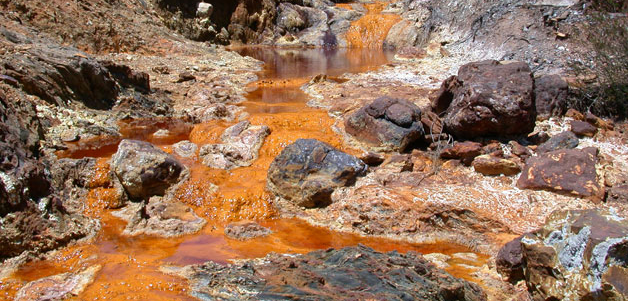
\includegraphics[width=0.6\textwidth]{figures/reactive-transport/mining.png}} \\
			\subfloat[Yellow slime mold]{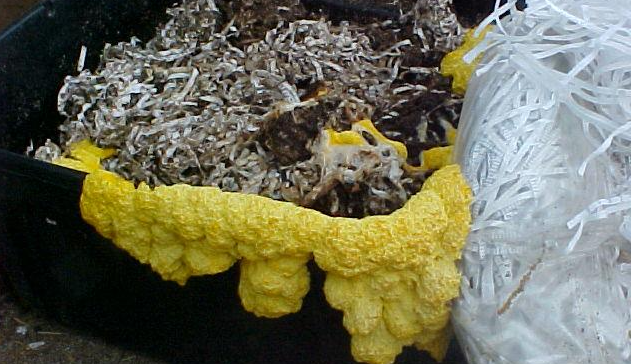
\includegraphics[width=0.6\textwidth]{figures/reactive-transport/biodegradation.png}} \\
			\subfloat[A landfill in Poland]{\includegraphics[width=0.6\textwidth]{figures/reactive-transport/landfill.png}}
		\end{figure}
	\end{columns}

	
\end{frame}
%%
%% --------------------------------------------------------------------------------------------------------------------%
%% Frontier research questions
%% --------------------------------------------------------------------------------------------------------------------%
%%
%\begin{frame}{Frontier research questions}
%	
%	\begin{itemize}
%		\item Pore scale and hybrid, or multiple continua, models capturing the scale dependence of coupled reactive transport processes.
%		\item Effects of chemical microenvironments. 
%		\item Coupled thermal-mechanical-chemical processes.
%		\item Control on mineral–fluid reaction rates in natural media. 
%		\item Scaling of reactive transport	processes from the microscopic to pore to field scale.
%		\item {\bf Example}: the \alert{\bf Critical Zone} (CZ) simulation\\
%			\begin{itemize}
%			\item a region with the low-temperature ($< 100 \, ^o$C) surface / near-surface environment where ``rock meets life''; 
%			\item water, atmosphere, rock, soil, and life interact creating the potential for complex chemical, physical, and biological interactions and responses to external forcing. 
%			\end{itemize}
%	\end{itemize}
%	
%\end{frame}
%
% --------------------------------------------------------------------------------------------------------------------%
% Example of coupled processes
% --------------------------------------------------------------------------------------------------------------------%
%
\begin{frame}{Example of coupled processes}
	
	\begin{figure}[!t]
		\centering
		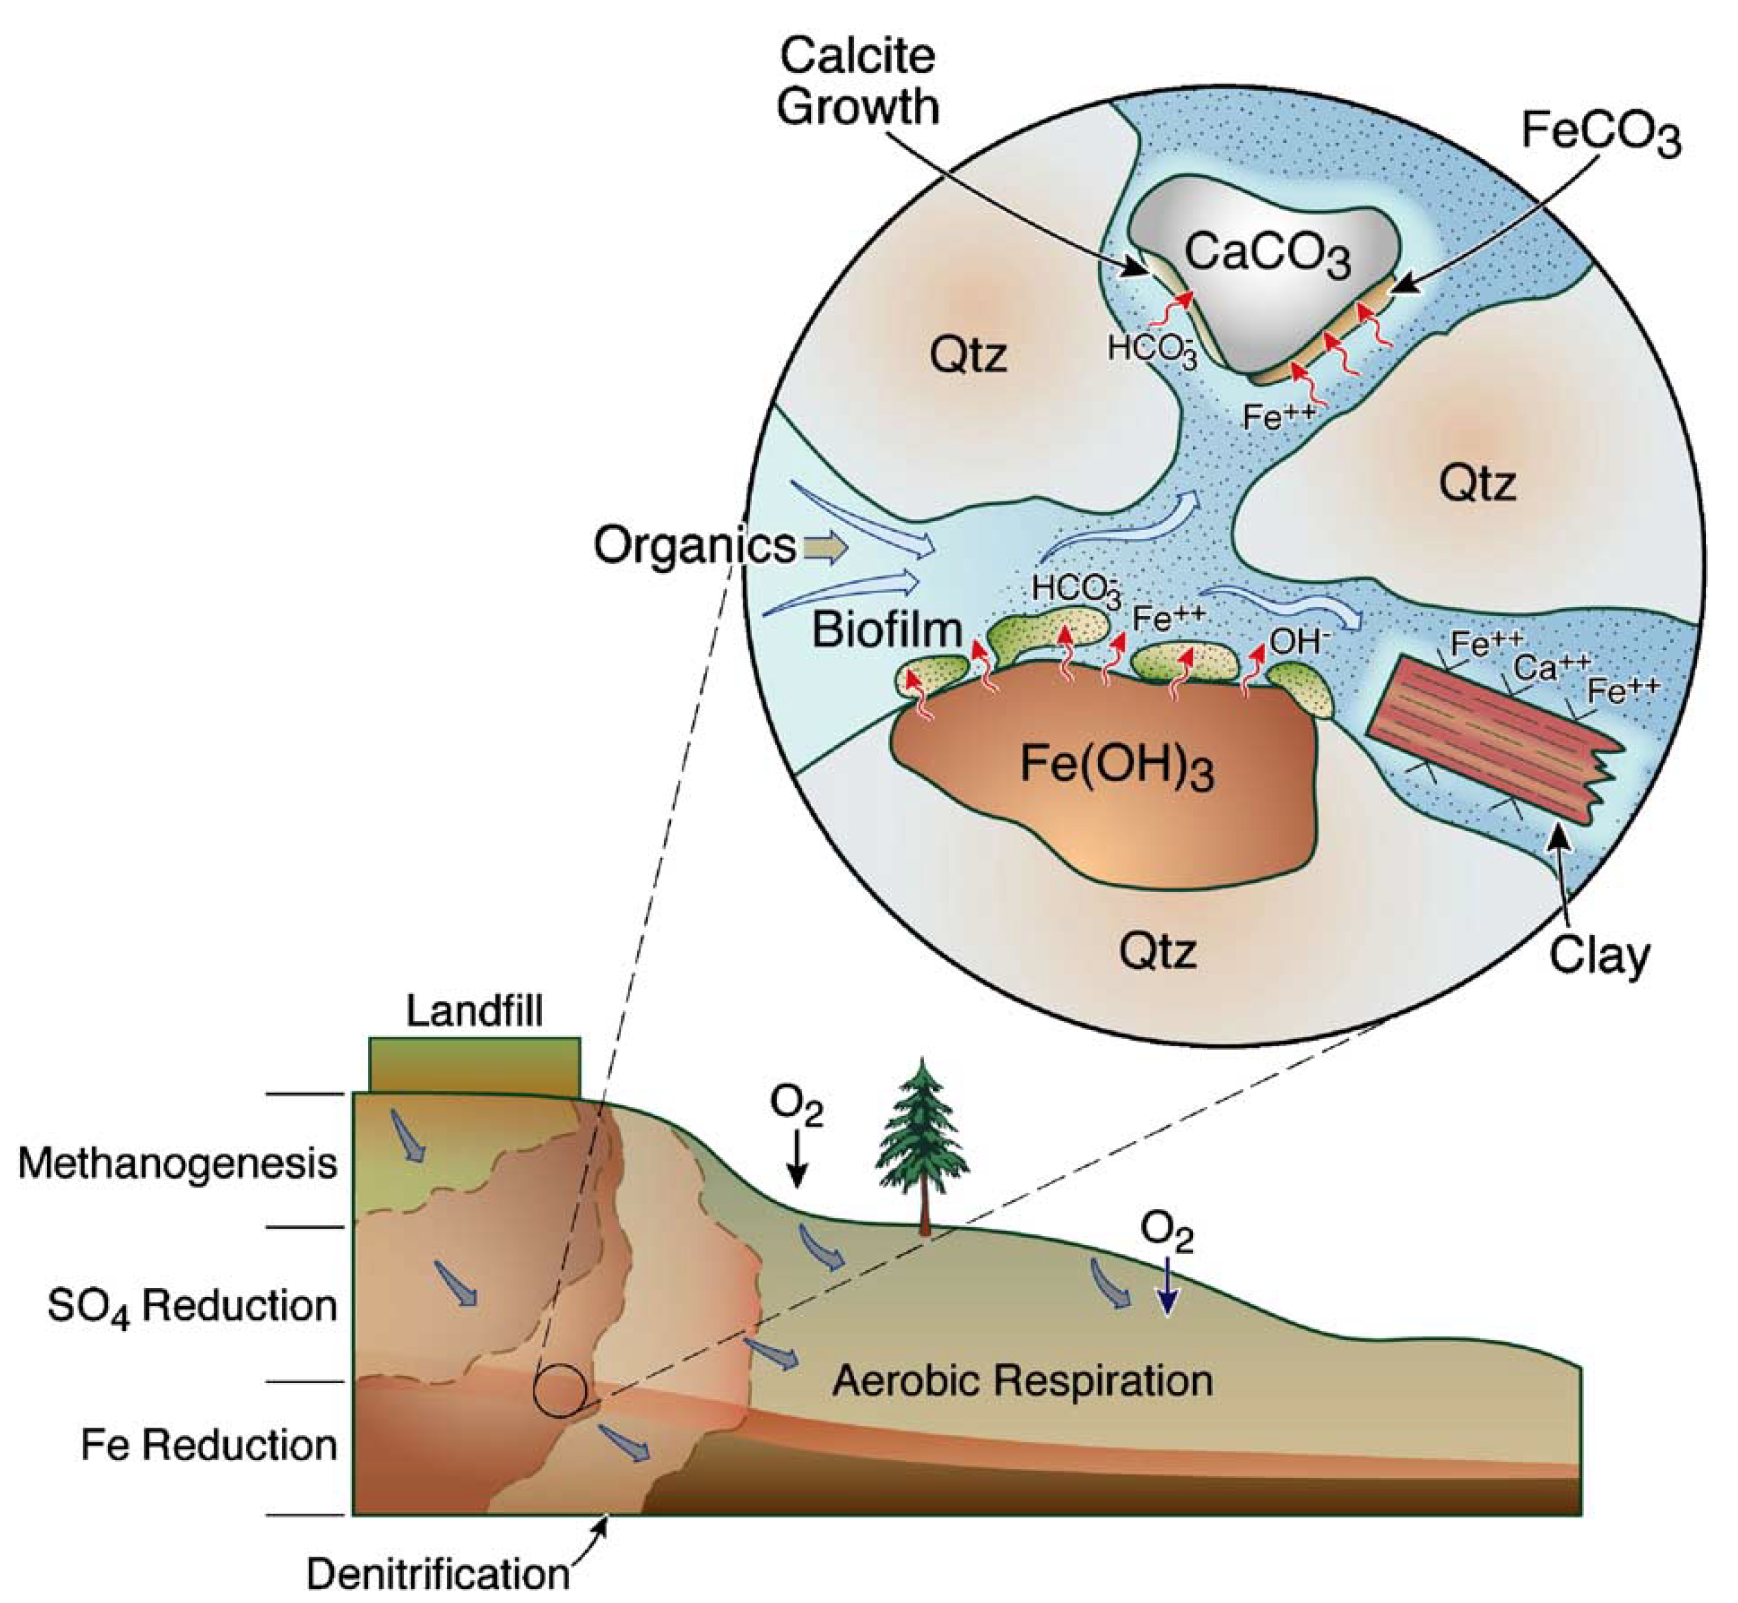
\includegraphics[width=0.47\textwidth]{figures/reactive-transport/steefel-coupling-example.png}
		\caption{Illustration from \cite{Steefel2005}: {\bf coupled geochemical, microbiological,
			and hydrologic processes operating at both the aquifer and pore scale}, i.e., oxidation-reduction zones developed in an aquifer downstream from an organic-rich landfill.}
	\end{figure}
	
	% https://www.e-education.psu.edu/png550/node/715
\end{frame}
%
% --------------------------------------------------------------------------------------------------------------------%
% Petroleum reservoir simulation
% --------------------------------------------------------------------------------------------------------------------%
%
\subsection{Petroleum reservoir simulation}
%
\begin{frame}{Petroleum reservoir simulation}
	
	
	
%	\begin{columns}[t]
%		\column{0.6\textwidth}
%		\vskip -5pt
	
		\begin{itemize}
		\item {\bf Important characteristics} of reservoir are the nature of the \alert{\bf rock and the fluids} filling it.
		%
		\pause
		\item \alert{\bf Reservoir characteristics}:
		\begin{itemize}
			\item heterogeneous;
			%
			\item properties heavily depend
			on the space location.
		\end{itemize}
		%
		\pause
		\item {\bf Example}: \alert{\bf fractured reservoir} is a set of heterogeneous porous media blocks (the matrix) and a net of fractures. {\bf Rock properties} (permeability) in such a reservoir dramatically change: 
		%
		\begin{itemize}
			\item permeability in the matrix is 1 millidarcy;
			\item permeability in the fractures is 1000 millidarcy.
		\end{itemize}

	\end{itemize}
		
%		\column{0.4\textwidth}
%		\vskip -20pt
%		
		\begin{figure}
			\centering
			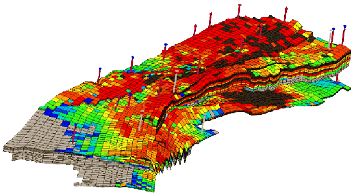
\includegraphics[width=0.4\textwidth]{figures/reactive-transport/reservoir-simulation.png}
		\end{figure}
%	\end{columns}

\end{frame}
%
% --------------------------------------------------------------------------------------------------------------------%
% Stages of oil recovery
% --------------------------------------------------------------------------------------------------------------------%
%
\begin{frame}{Stages of oil recovery}
	The nature of the fluids filling in reservoir strongly depends on the \alert{\bf stage of oil recovery}:
	\begin{itemize}
		\item {\bf Early stage / primary recovery}: 
		\begin{itemize}
			\item single fluid (gas/oil), 
			\item high pressure,
			\item gas/oil is produced by natural decompression without 
			pumping effort at the wells, 
			\item stage ends when a pressure equilibrium between the oil field and the atmosphere occurs.
		\end{itemize}
		\item {\bf Secondary recovery stage} (to recover part of the remaining oil): 
		\begin{itemize}
			\item fluid is injected through injection wells,
			\item oil is produced through production wells,
			\item high reservoir pressure,
			\item high flow rates,
			\item 
			$
			\begin{cases}
			P_{\rm reservior} \geq P_{\rm bubble}: & 
			\text{two-phase immiscible flow (water and oil phases),} \\
			P_{\rm reservior} < P_{\rm bubble}: & 	
			\text{the flow is of the oil type.} \\
			%\text{the oil splits into liquid and gaseous phases;} \\
			%& 	\text{the water phase does not exchange mass with the other phases, but the liquid and gaseous phases exchange mass} \\
			\end{cases}
			$			
		\end{itemize}
		%
	\end{itemize}
\end{frame}
%
% --------------------------------------------------------------------------------------------------------------------%
% Enhanced oil recovery techniques
% --------------------------------------------------------------------------------------------------------------------%
%
\begin{frame}{Enhanced oil recovery techniques}
	\begin{itemize}
	 \item \alert{\bf Water flooding}
	 %
	\begin{itemize}
		\item is not very effective:  $> 50 \%$  of hydrocarbons often remain in the reservoir;
		%
		\item large amount of oil is trapped in small pores and cannot be washed out;
		%
		\item the oil is heavy and viscous, whereas the water is extremely mobile $\Rightarrow$
		%
		
		with sufficiently high flow rates, the production wells primarily produce water instead of oil.
	\end{itemize}
	%
	\item \alert{\bf Enhanced recovery techniques} (using complex chemical and thermal effects) is injecting materials that are not normally present in a petroleum reservoir. 
	%
	\item {\bf Main objective} of these techniques	is to achieve \alert{\bf miscibility} (and thus \alert{\bf eliminate the residual oil saturation oil}) by
	%
	\begin{itemize}
		\item increasing temperature (e.g., in situ combustion) or
		\item injecting other chemical species (e.g., CO$_2$).
	\end{itemize}
	%
	\item Popular enhanced recovery techniques: 
		\begin{itemize}
			\item {\bf composition flow} (given chemical composition, the rest is dependent on the thermodynamic conditions and the overall concentration of each species);
			\item {\bf thermal methods} (steam drive and soak);
			\item {\bf chemical flooding} (alkaline, surfactant, polymer, and foam flooding).
		\end{itemize}
	\end{itemize}
\end{frame}
% --------------------------------------------------------------------------------------------------------------------%
% Advection--diffusion equation (transport equation)
% --------------------------------------------------------------------------------------------------------------------%
%
%
\subsection{Advection-diffusion-reaction equation}
\begin{frame}{Advection-diffusion-reaction equation (transport equation) \, i}
\begin{itemize}
\item Conservation laws permit us to derive the following partial differential
equation that governs the {\bf transport of a conservative quantity} $u$:
%
{
	\small
	\begin{align*}
		\frac{\partial u}{\partial t}+\nabla\cdot(\boldsymbol{v}u-D\nabla u) + \rho (u) & =f &  & \boldsymbol{x}\in\Omega,\;t>0
%		\\[-5pt]
%		u & =u_{0} & \vphantom{\frac{\partial u}{\partial t}} & \boldsymbol{x}\in\Omega,\;t=0\\[-5pt]
%		u & =u_{D} & \vphantom{\frac{\partial u}{\partial t}} & \boldsymbol{x}\in\Gamma_{D},\;t>0\\[-5pt]
%		\boldsymbol{v}u-D\nabla u & =g & \vphantom{\frac{\partial u}{\partial t}} & \boldsymbol{x}\in\Gamma_{N},\;t>0,
	\end{align*}
}
%
	\item \alert{\bf Quiz}: which operator in this equation could be responsible for the reactive part of the modeling?
	%
	\begin{center}
		\href{http://etc.ch/YYq6}{\textcolor{indigo(dye)}{\tt http://etc.ch/YYq6}} \quad or \quad 
		
\includegraphics[height=0.2\columnwidth]{figures/reactive-transport/polls.png}
	\end{center}
	\item \alert{\bf Answer}: $\rho (u)$ is the non-linear reaction function. 
%where \\[5pt]
%
%\begin{itemize}
%	\item $\frac{\partial u}{\partial t}$ is the  \alert{\bf time derivative};\\[2pt]
%	%
%	\item $\nabla u = \begin{pmatrix}\tfrac{\partial u}{\partial x} & \tfrac{\partial u}{\partial y} & \tfrac{\partial u}{\partial z}\end{pmatrix} $ is the \alert{\bf gradient operator} of scalar variable $u$ denoting \alert{\bf flux} and in combination with $D$ accounting for the \alert{\bf diffusion/dispersion processes}; \\[2pt]
%	%
%	\item $\nabla\cdot\boldsymbol{v} =\tfrac{\partial v_{x}}{\partial x}+\tfrac{\partial v_{y}}{\partial y}+\tfrac{\partial v_{z}}{\partial z}$ is the \alert{divergence operator} of vector
%	variable $\boldsymbol{v}$ accounting \alert{\bf convection/advection};\\[2pt]
%	%
%	\item $\rho (u)$ is the \alert{\bf reaction operator}. 
%\end{itemize}
\end{itemize}
%
\end{frame}
\begin{frame}{Advection-diffusion-reaction equation (transport equation) \, ii}
	\begin{itemize}
		\item Conservation laws permit us to derive the following partial differential
		equation that governs the {\bf transport of a conservative quantity} $u$:
		%
		{
			\small
			\begin{align*}
				\frac{\partial u}{\partial t}+\nabla\cdot(\boldsymbol{v}u-D\nabla u) + \rho (u) & =f &  & \boldsymbol{x}\in\Omega,\;t>0
				%		\\[-5pt]
				%		u & =u_{0} & \vphantom{\frac{\partial u}{\partial t}} & \boldsymbol{x}\in\Omega,\;t=0\\[-5pt]
				%		u & =u_{D} & \vphantom{\frac{\partial u}{\partial t}} & \boldsymbol{x}\in\Gamma_{D},\;t>0\\[-5pt]
				%		\boldsymbol{v}u-D\nabla u & =g & \vphantom{\frac{\partial u}{\partial t}} & \boldsymbol{x}\in\Gamma_{N},\;t>0,
			\end{align*}
		}
	   %
		where \\[5pt]
		%
		\begin{itemize}
			\item $\frac{\partial u}{\partial t}$ is the  \alert{\bf time derivative};\\[2pt]
			%
			\item $\nabla u = \begin{pmatrix}\tfrac{\partial u}{\partial x} & \tfrac{\partial u}{\partial y} & \tfrac{\partial u}{\partial z}\end{pmatrix} $ is the \alert{\bf gradient operator} of scalar variable $u$ denoting the  \alert{\bf flux} and in combination with $D$ accounting for the \alert{\bf diffusion/dispersion processes}; \\[2pt]
			%
			\item $\nabla\cdot\boldsymbol{v} =\tfrac{\partial v_{x}}{\partial x}+\tfrac{\partial v_{y}}{\partial y}+\tfrac{\partial v_{z}}{\partial z}$ is the \alert{\bf divergence operator} of vector
			variable $\boldsymbol{v}$ accounting \alert{\bf convection/advection};\\[2pt]
			%
			\item $\rho (u)$ is the \alert{\bf reaction operator}. 
		\end{itemize}
	\end{itemize}
\end{frame}
%
% --------------------------------------------------------------------------------------------------------------------%
% Advection-diffusion-reaction initial boundary value problem (I-BVP)
% --------------------------------------------------------------------------------------------------------------------%
%
\begin{frame}{Advection-diffusion-reaction initial boundary value problem (I-BVP)}

\begin{itemize}
\item With initial and boundary condition, 
we obtain \alert{\bf initial boundary value problem (I-BVP)}
%
\begin{align*}
\partial u/\partial t+\nabla\cdot(\boldsymbol{v}u-D\nabla u)  + \rho (u) & =f &  & \boldsymbol{x}\in\Omega,\;t>0\\
u & =u_{0} &  & \boldsymbol{x}\in\Omega,\;t=0\\
u & =u_{D} &  & \boldsymbol{x}\in\Gamma_{D},\;t>0\\
\boldsymbol{v}u-D\nabla u & =g &  & \boldsymbol{x}\in\Gamma_{N},\;t>0
\end{align*}
%
\vskip -5pt
\begin{itemize}
\item $u$ is some \alert{conservative quantity} (e.g., energy, species
amounts) per volume;
\item $\boldsymbol{v}$ is the \alert{velocity field} in which the quantity is advected;
\item $D$ is a \alert{dispersion–diffusion tensor}; 
%a coefficient that controls diffusion/dispersion rates};
\item $f$ is a \alert{rate of generation} (e.g., heat generation, reaction
rate).
\item $u_{0}$ is the \emph{given} \alert{initial condition} of $u$ at
time $t=0$ at every $x$ in the domain $\Omega$;
\item $u_{D}$ is the \emph{given} value of $u$ on a \alert{Dirichlet boundary}
$\Gamma_{D}$;
\item $g$ is the \emph{given} value of the flux $\boldsymbol{v}u-D\nabla u$
on a \alert{Neumann boundary} $\Gamma_{N}$.
\end{itemize}
\end{itemize}

\end{frame}
%
% --------------------------------------------------------------------------------------------------------------------%
% Exercise: one-dimensional advection-diffusion equation
% --------------------------------------------------------------------------------------------------------------------%
%
\begin{frame}{Exercise, 1D advection-diffusion equation}
\begin{itemize}
\item \alert{\textbf{Exercise:}} Write the partial differential equation
\[
\frac{\partial u}{\partial t}+\nabla\cdot(\boldsymbol{v}u-D\nabla u)  + \rho (u) =f
\]
for the \textbf{one dimensional case} with $u=u(t,x)$ and a scalar velocity $v$. 
\hiddenpause
\item \textbf{Answer:} one dimensional case of the equation above reads as follows:
%
\[
\frac{\partial u}{\partial t}+\frac{\partial}{\partial x}\left(vu-D\frac{\partial u}{\partial x}\right)  + \rho (u) =f.
\]
Alternatively, we can apply the operator $\partial/\partial x$ on
each term inside parenthesis to get 
\[
\frac{\partial u}{\partial t}+\frac{\partial(vu)}{\partial x}-\frac{\partial}{\partial x}\left(D\frac{\partial u}{\partial x}\right)  + \rho (u) = f.
\]
\end{itemize}
\end{frame}
%
% --------------------------------------------------------------------------------------------------------------------%
% Exercise: one-dimensional advection-diffusion equation with constant diffusion and velocity
% --------------------------------------------------------------------------------------------------------------------%
%
\begin{frame}{Exercise, 1D advection-diffusion equation (constant diffusion and velocity)}
\begin{itemize}
\item \alert{\textbf{Quiz:}} Giving which assumptions can you simplify
\[
\frac{\partial u}{\partial t}+\frac{\partial(vu)}{\partial x}-\frac{\partial}{\partial x}\left(D\frac{\partial u}{\partial x}\right)+ \rho (u) =f?
\]
%
to 
%
\[
\frac{\partial u}{\partial t}+v\frac{\partial u}{\partial x}-D\frac{\partial^{2}u}{\partial x}+ \rho (u) =f.
\]
\begin{center}
		\href{http://etc.ch/YYq6}{\textcolor{indigo(dye)}{\tt http://etc.ch/YYq6}} \quad or \quad 
		
\includegraphics[height=0.2\columnwidth]{figures/reactive-transport/polls.png}
	\end{center}
\hiddenpause
\item \alert{\textbf{Answer}}: Both $v$ and $D$ must be constant.
\end{itemize}
\end{frame}
%
% --------------------------------------------------------------------------------------------------------------------%
% Numerical solution of the transport equations
% --------------------------------------------------------------------------------------------------------------------%
%
\begin{frame}{First-order splitting to transport and reaction equations}
	\begin{itemize}
		\item Let us represent 
		%
		\[\frac{\partial u}{\partial t}+\nabla\cdot(\boldsymbol{v}u-D\nabla u)  + \rho (u) = 0 \qquad \text{as} \qquad \frac{\partial u}{\partial t}+T(u) + R(u) = 0\] 
		%
		where \alert{\bf $T(u)$ and $R(u)$ are transport and reaction operators}.\\[10pt]
		%
		\pause
		\item According to the \alert{\bf first-order splitting}, we first solve the {\bf transport equation} for $\bar{u}$, i.e., 
		%		
		\begin{alignat*}{2}
		\frac{\partial \bar{u}}{\partial t}+T(\bar{u}) & = 0, \quad \;\: t > 0, \\[-5pt]
		\bar{u} &= u_0, \quad  t = 0, 
		\end{alignat*}
		%
		and next the {\bf reaction equation} with reconstructed $\bar{u}$ as the initial condition, i.e.,  
		%
		\begin{alignat*}{2}
			\frac{\partial u}{\partial t}+R(u) & = 0, \quad  t > 0, \\[-5pt]
			u & = \bar{u}, \quad  t = 0. 
		\end{alignat*}
	\end{itemize}
\end{frame}
%
% --------------------------------------------------------------------------------------------------------------------%
% Numerical solution of the transport equations
% --------------------------------------------------------------------------------------------------------------------%
%
\begin{frame}{Reaction equation in terms of chemical kinetic-equilibrium problem}
	\begin{itemize}
		\item{\bf Reaction equation} 
		%
		\begin{alignat*}{2}
			\tfrac{\partial u}{\partial t}+R(u) & = 0, \quad  t > 0, \\[-5pt]
			u & = \bar{u}, \quad  t = 0,
		\end{alignat*}
		% 
		is already discussed \alert{\bf chemical kinetic-equilibrium differential-algebraic equation (DAE)} 
		%
		\begin{alignat*}{4}
			\tfrac{\mathrm{d}b_{e}}{\mathrm{d}t} & = f_e(n_e), %A_{e}(q_{e}+\nu_{e}^{{\rm T}}r)
			& \quad  &  t > 0, \\
			\tfrac{\mathrm{d}n_{k}}{\mathrm{d}t} & = f_k(n_k),
			%\nu_{k}^{{\rm T}}r+q_{k} 
			&  \quad & t>0, \\
			n_{e}  & = \varphi(T,P,b_{e}), & \quad  &  t > 0, \\
			b_{e}  & = An_{e}^{\circ},       & \quad  & t = 0, \\
			n_{k}  & = n_{k}^{\circ},         & \quad  & t=0.			
		\end{alignat*}
		%
		solved by the scheme suitable for the stiff systems of ODEs and GEM approach.
	\end{itemize}
	
\end{frame}
%
% --------------------------------------------------------------------------------------------------------------------%
% Numerical solution of the transport equations
% --------------------------------------------------------------------------------------------------------------------%
%
\begin{frame}{Numerical solution of the transport equations}
\begin{itemize}
\item There are many {\bf numerical methods for the solution of the I-BVP} with transport equation \\[-15pt]
%
\[
\frac{\partial u}{\partial t}+T(u) = f.
\]
%\item Most commonly used ones are \alert{finite difference (FD)}, \alert{finite volume (FV)}, and \alert{finite element (FE)} methods.
%\begin{itemize}
%	\item \alert{finite difference (FD)}, 
%	\item \alert{finite volume (FV)}, and 
%	\item \alert{finite element (FE)} methods.
%\end{itemize}
%
\vskip -15pt
\pause
\item \alert{\bf Finite difference method (FDM)}:
\begin{itemize}
	\item is the {\bf simplest} of all methods, 
	\item has {\bf disadvantages} when \alert{complex geometries} are involved.
\end{itemize}
%\begin{mylist}
%	\small
%	\item is the {\bf simplest} of all methods,
%	\itema has {\bf disadvantages} in case of {\bf complex geometries}.
%\end{mylist}
%
\pause
\item \alert{\bf Finite volume method (FVM)}:
\begin{itemize}
	\item forces {\bf conservation of quantities} at discretized level, 
	\item only needs to do flux evaluation for the cell boundaries,
	\item can be used on {\bf unstructured (triangular) grids}, 
	\item {\bf the higher-order approximations} are not easily constructed.
\end{itemize}
%\begin{mylist}
%	\small
%	\item forces {\bf conservation of quantities} at discretized level, 
%	\item only needs to do flux evaluation for the cell boundaries,
%	\item can be used on {\bf unstructured (triangular) grids}, 
%	\itema {\bf the higher-order approximations} are not easily.
%\end{mylist}
%\begin{itemize}
%	\item is the {\bf simplest} of all methods, 
%	\item has {\bf disadvantages} when \alert{complex geometries} are involved.
%\end{itemize}
%
\pause
\item \alert{\bf Finite element method (FEM)}:
%\begin{mylist}
%	\small
%	\item applicable for {\bf general boundary conditions, complex geometry, and  variable material properties},
%	\item clear {\bf structure and versatility} (e.g., mixed formulation), 
%	\item solid theoretical base to obtain {\bf error estimates}.
%\end{mylist}
\begin{itemize}
	\item applicable to {\bf general boundary conditions}, {\bf complex geometry}, and {\bf variable material properties},
	\item clear {\bf structure and versatility} (e.g., mixed formulation), 
	\item solid theoretical base to obtain {\bf error estimates}.
\end{itemize}
%

\end{itemize}
\end{frame}
%
% --------------------------------------------------------------------------------------------------------------------%
% Basics of finite difference method
% --------------------------------------------------------------------------------------------------------------------%
%
\begin{frame}{Basics of finite difference method (FDM)}
\begin{itemize}
\item In the \alert{\bf FDM}, the derivatives are approximated
with {\bf finite difference formulas}.
\pause
\item The \alert{\bf Taylor expansion} is a \textbf{polynomial} approximation of function $f$ around
a point $x_{i}$
\[
f(x_{i}+\Delta x)=f(x_{i})+\frac{\partial f(x_{i})}{\partial x}\,\Delta x+\frac{1}{2}\frac{\partial^{2}f(x_{i})}{\partial x^{2}}\,\Delta x^{2}+\cdots+\frac{1}{n!}\frac{\partial^{n}f(x_{i})}{\partial x^{n}}\,\Delta x^{n}+\cdots
\]
\pause
\item \alert{\textbf{Quiz:}} what is the Taylor expansion for $f(x)=e^{x}$ around
$x_{i}=0$

\begin{center}
		\href{http://etc.ch/YYq6}{\textcolor{indigo(dye)}{\tt http://etc.ch/YYq6}} \quad or \quad 
		
\includegraphics[height=0.1\columnwidth]{figures/reactive-transport/polls.png}
	\end{center}
%
\hiddenpause
\item \textbf{Answer:}
\[
f(x_{i}+\Delta x)=e^{x_{i}+\Delta x} \approx 1+\, \Delta x+\frac{1}{2}\, \Delta x^{2}+\frac{1}{6}\, \Delta x^{3}+\cdots
\]
\end{itemize}
\end{frame}
%
% --------------------------------------------------------------------------------------------------------------------%
% Approximation of e using Taylor series
% --------------------------------------------------------------------------------------------------------------------%
%
\begin{frame}{Approximation of $\boldsymbol{e^{\boldsymbol{x}}}$ using Taylor series}
\begin{center}
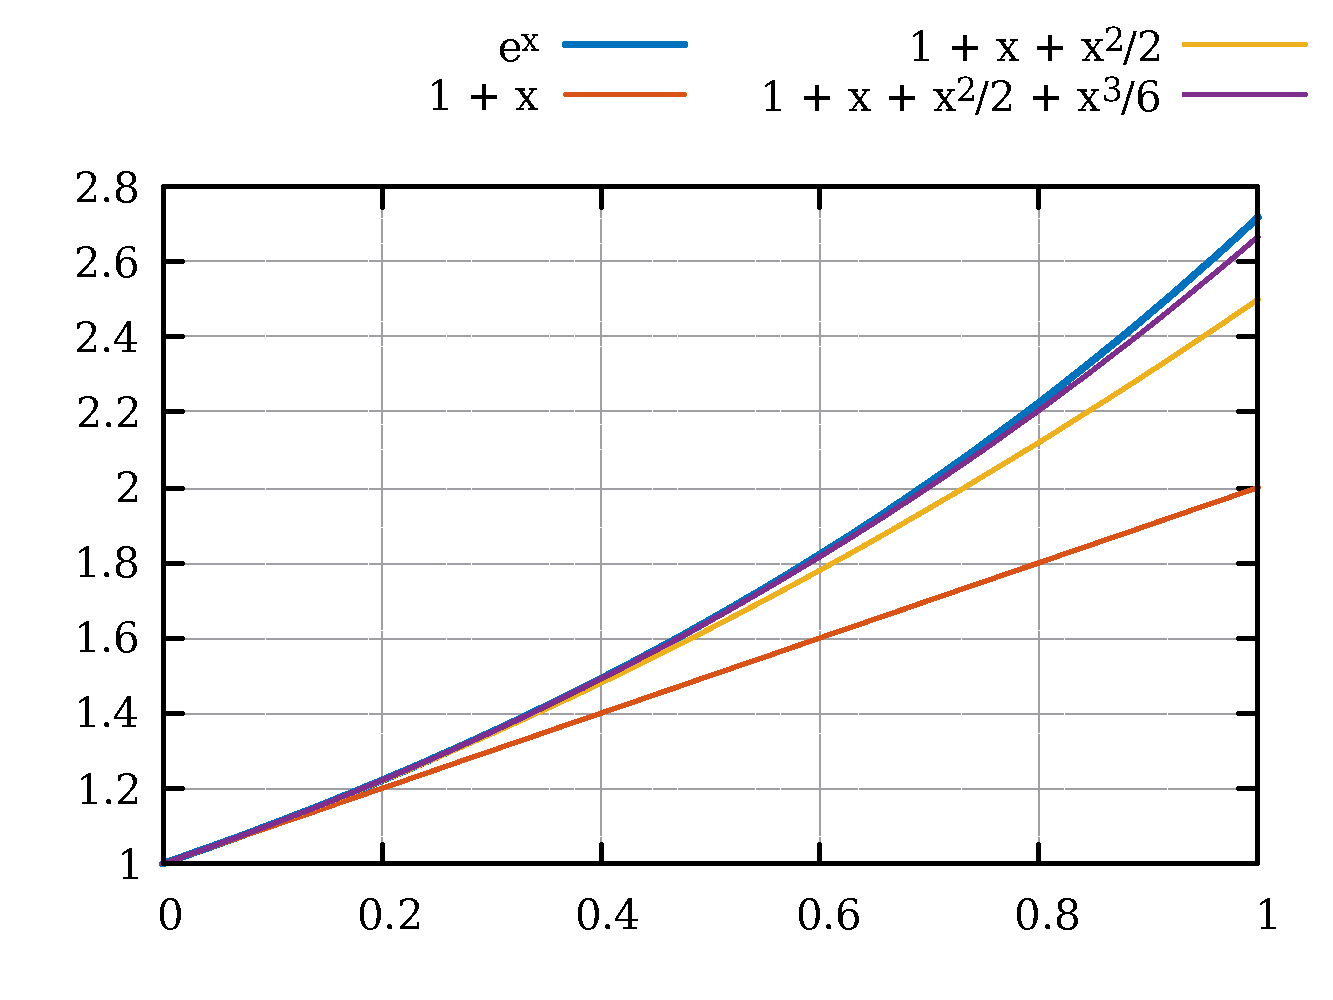
\includegraphics[height=0.9\textheight]{figures/reactive-transport/taylor-expansion-exp}
%\caption{}
\par\end{center}

\end{frame}
%
% --------------------------------------------------------------------------------------------------------------------%
% First-order FDM scheme
% --------------------------------------------------------------------------------------------------------------------%
%
\begin{frame}{First-order FDM scheme}
\begin{itemize}
\item We can derive \alert{\textbf{finite difference approximations}} for derivatives 
$\frac{\partial f(x_{i})}{\partial x}$, $\frac{\partial^{2}f(x_{i})}{\partial x^{2}}$, etc: 
%
% by truncating the Taylor expansion 
% \[
% f(x_{i}+\Delta x)=f(x_{i})+\frac{\partial f(x_{i})}{\partial x}\,\Delta x+\frac{1}{2}\frac{\partial^{2}f(x_{i})}{\partial x^{2}}\,\Delta x^{2}+\cdots+\frac{1}{n!}\frac{\partial^{n}f(x_{i})}{\partial x^{n}}\,\Delta x^{n}+\cdots
% \]
% %
% up until the \alert{derivative order}. 
\item {\bf 1st order approximation of $\frac{\partial f(x_{i})}{\partial x}$ }
\[
{\displaystyle \frac{\partial f(x_{i})}{\partial x}\approx\frac{f(x_{i}+h)-f(x_{i})}{\Delta x}} + O (\Delta x),
\]
%
\item {\bf 2nd order approximation} (central difference) of $\frac{\partial f(x_{i})}{\partial x}$ 
%
\[
\frac{\partial f(x_{i})}{\partial x}\approx\frac{f(x_{i}+\Delta x)-f(x_{i}-\Delta x)}{2\Delta x}+O(\Delta x^{2})
\]
%
\item {\bf 2nd order approximation} of $\frac{\partial^{2}f(x_{i})}{\partial x^{2}}$ 
%
\[
\frac{\partial^{2}f(x_{i})}{\partial x^{2}} \approx\frac{f(x_{i}+\Delta x)-2f(x_{i})+f(x_{i}-\Delta x)}{\Delta x^{2}}
\]
%
% the error decrease is of order $O (h)$ with decreasing $h$.
%
% \pause
% \item \alert{\textbf{Exercise:}} Derive the {\bf second order approximation}, where the approximation error is proportional to $O(h^{2})$ with a decrease of $h$?
% %
\end{itemize}
\end{frame}
% --------------------------------------------------------------------------------------------------------------------%
% Second-order FDM scheme
% --------------------------------------------------------------------------------------------------------------------%
%
% \begin{frame}{Second-order FDM scheme, Central difference approximation}
% \begin{itemize}
% \item Write the following two {\bf truncated Taylor expansions}:
% \begin{align*}
% f(x_{i}+\Delta x) & =f(x_{i})+\frac{\partial f(x_{i})}{\partial x}\Delta x+\frac{1}{2}\frac{\partial^{2}f(x_{i})}{\partial x^{2}}\Delta x^{2}+O(\Delta x^{3})\\
% f(x_{i}-\Delta x) & =f(x_{i})-\frac{\partial f(x_{i})}{\partial x}\Delta x+\frac{1}{2}\frac{\partial^{2}f(x_{i})}{\partial x^{2}}\Delta x^{2}+O(\Delta x^{3})
% \end{align*}
% %
% \pause
% \item By subtracting the two equations, we can write
% \[
% \frac{\partial f(x_{i})}{\partial x}\approx\frac{f(x_{i}+\Delta x)-f(x_{i}-\Delta x)}{2\Delta x}+O(\Delta x^{2})
% \]
% which is a \alert{\bf central finite difference approximation} for $\partial f(x_{i})/\partial x$.
% \end{itemize}
% \end{frame}
%
% --------------------------------------------------------------------------------------------------------------------%
% Basics of finite difference method
% --------------------------------------------------------------------------------------------------------------------%
%
% \begin{frame}{Usage of FDM to transform differential equation}
% \begin{itemize}
% \item We use the \alert{\bf finite difference formulas}
% \begin{align*}
% \frac{\partial f(x_{i})}{\partial x} & \approx\frac{f(x_{i}+\Delta x)-f(x_{i}-\Delta x)}{2\Delta x}\\
% \shortintertext{and}
% \frac{\partial^{2}f(x_{i})}{\partial x^{2}} & \approx\frac{f(x_{i}+\Delta x)-2f(x_{i})+f(x_{i}-\Delta x)}{\Delta x^{2}}
% \end{align*}
% to transform the \textbf{partial differential equation} (PDE)
% \[
% \frac{\partial u}{\partial t}+v\frac{\partial u}{\partial x}-D\frac{\partial^{2}u}{\partial x}=f \quad \mbox{on} \quad [x_L, x_R]
% \]
% into a \textbf{system of linear algebraic equations}.
% \end{itemize}
% \end{frame}
%
% --------------------------------------------------------------------------------------------------------------------%
% Discretization of the transport equations
% --------------------------------------------------------------------------------------------------------------------%
%
\begin{frame}{Discretization of transport equation, Computational domain discretization}
\begin{itemize}
\item We \alert{numerically solve} the transport problem
\begin{alignat*}{4}
\frac{\partial u}{\partial t}+v\frac{\partial u}{\partial x}-D\frac{\partial^{2}u}{\partial x} & =f &  x_L <x<x_R, &\quad t>0,\\
u & =0\qquad \vphantom{\frac{\partial^{2}u}{\partial x}} & x_L< x <x_R, & \quad t=0,\\
u & =1 \vphantom{\frac{\partial^{2}u}{\partial x}} & x=x_L,& \quad t>0,
\end{alignat*}
and free boundary at $x=x_R$ using the \alert{finite difference method (FDM)}.\\[5pt]
%
\item Consider the following \textbf{uniform discretization} of computational  domain $[x_L, x_R]$:
\end{itemize}
%
\vskip 20pt
\begin{center}
\includegraphics[width=0.8\textwidth]{figures/reactive-transport/finite-difference-domain-discretization}
\end{center}

\end{frame}
%
% --------------------------------------------------------------------------------------------------------------------%
% Discretization of the transport equations
% --------------------------------------------------------------------------------------------------------------------%
%
\begin{frame}{Discretization of transport equation, Finite difference formulas}

\begin{itemize}
\item Using \alert{\bf finite difference formulas}, we can approximate the partial derivatives in transport equation as follows:
%
\begin{alignat*}{2}
\frac{\partial u}{\partial t} & \approx\frac{u_{i}^{k+1}-u_{i}^{k}}{\Delta t} & \qquad & x=x_{i},\;t=t_{k}\\
\frac{\partial u}{\partial x} & \approx\frac{u_{i+1}^{k+1}-u_{i-1}^{k+1}}{2\Delta x} & \qquad & x=x_{i},\;t=t_{k}\\
\frac{\partial^{2}u}{\partial x^2} & \approx\frac{u_{i+1}^{k+1}-2u_{i}^{k+1}+u_{i-1}^{k+1}}{\Delta x^{2}} & \qquad & x=x_{i},\;t=t_{k}
\end{alignat*}
\end{itemize}

\vskip 20pt
\begin{center}
	\includegraphics[width=0.8\textwidth]{figures/reactive-transport/finite-difference-domain-discretization}
\end{center}

\end{frame}
%
% --------------------------------------------------------------------------------------------------------------------%
% Discretization of the transport equations
% --------------------------------------------------------------------------------------------------------------------%
%
\begin{frame}{Discretization of transport equation: system of algebraic equations}

\small
\begin{itemize}
\item The differential equation
\[
\frac{\partial u}{\partial t}+v\frac{\partial u}{\partial x}-D\frac{\partial^{2}u}{\partial x}=f
\]
%
\vskip 10pt
becomes a \textbf{system of algebraic equations}
\[
\left(\frac{u_{i}^{k+1}-u_{i}^{k}}{\Delta t}\right)+v\left(\frac{u_{i+1}^{k+1}-u_{i-1}^{k+1}}{2\Delta x}\right)-D\left(\frac{u_{i+1}^{k+1}-2u^{k+1}_{i}+u_{i-1}^{k+1}}{\Delta x^{2}}\right)=f_{i}\quad(i=1,\ldots,n-1)
\]
\item With {\bf recovered values} $u^k_i$ ($u$ on every \alert{discrete point} $x_{i}$ at \alert{discrete time} $t_{k}$), we solve algebraic equations to find \alert{$u^{k+1}_i$} ($u$ on every $x_{i}$ at ${t_{k+1}=t_{k}+\Delta t}$):\\[10pt]
\end{itemize}
%
\[
\alert{u_{i}^{k+1}}
+ \frac{v \, \Delta t}{2\Delta x} \left(\alert{u_{i+1}^{k+1}}-\alert{u_{i-1}^{k+1}}\right)
- \frac{D \, \Delta t}{\Delta x^{2}} \left(\alert{u_{i+1}^{k+1}}-2\,\alert{u^{k+1}_{i}}+\alert{u_{i-1}^{k+1}}\right) 
= \Delta t \, f_{i} + u_{i}^{k} \quad(i=1,\ldots,n-1)
\]

%\begin{center}
%\includegraphics[width=0.8\textwidth]{figures/reactive-transport//finite-difference-domain-discretization}
%\par\end{center}

\end{frame}
%
% --------------------------------------------------------------------------------------------------------------------%
% Discretization of the transport equations
% --------------------------------------------------------------------------------------------------------------------%
%
\begin{frame}{Discretization of transport equation: central vs. upwind scheme}

\lcol
\begin{itemize}
\item The \alert{\bf central scheme} for the finite difference approximation
of the advection term, i.e., 
\[
v\, \frac{\partial u}{\partial x}\approx 
v\, \left(\frac{u_{i+1}^{k+1}-u_{i-1}^{k+1}}{2\Delta x}\right),
\]
can produce \alert{spurious oscillations}.
%
\item One can use instead an \alert{\bf upwind scheme}, i.e., 
\[
v\, \frac{\partial u}{\partial x}\approx 
v\, \left(\frac{u_{i}^{k+1}-u_{i-1}^{k+1}}{\Delta x}\right),
\]
to prevent this. 

\end{itemize}
\rcol
\begin{center}
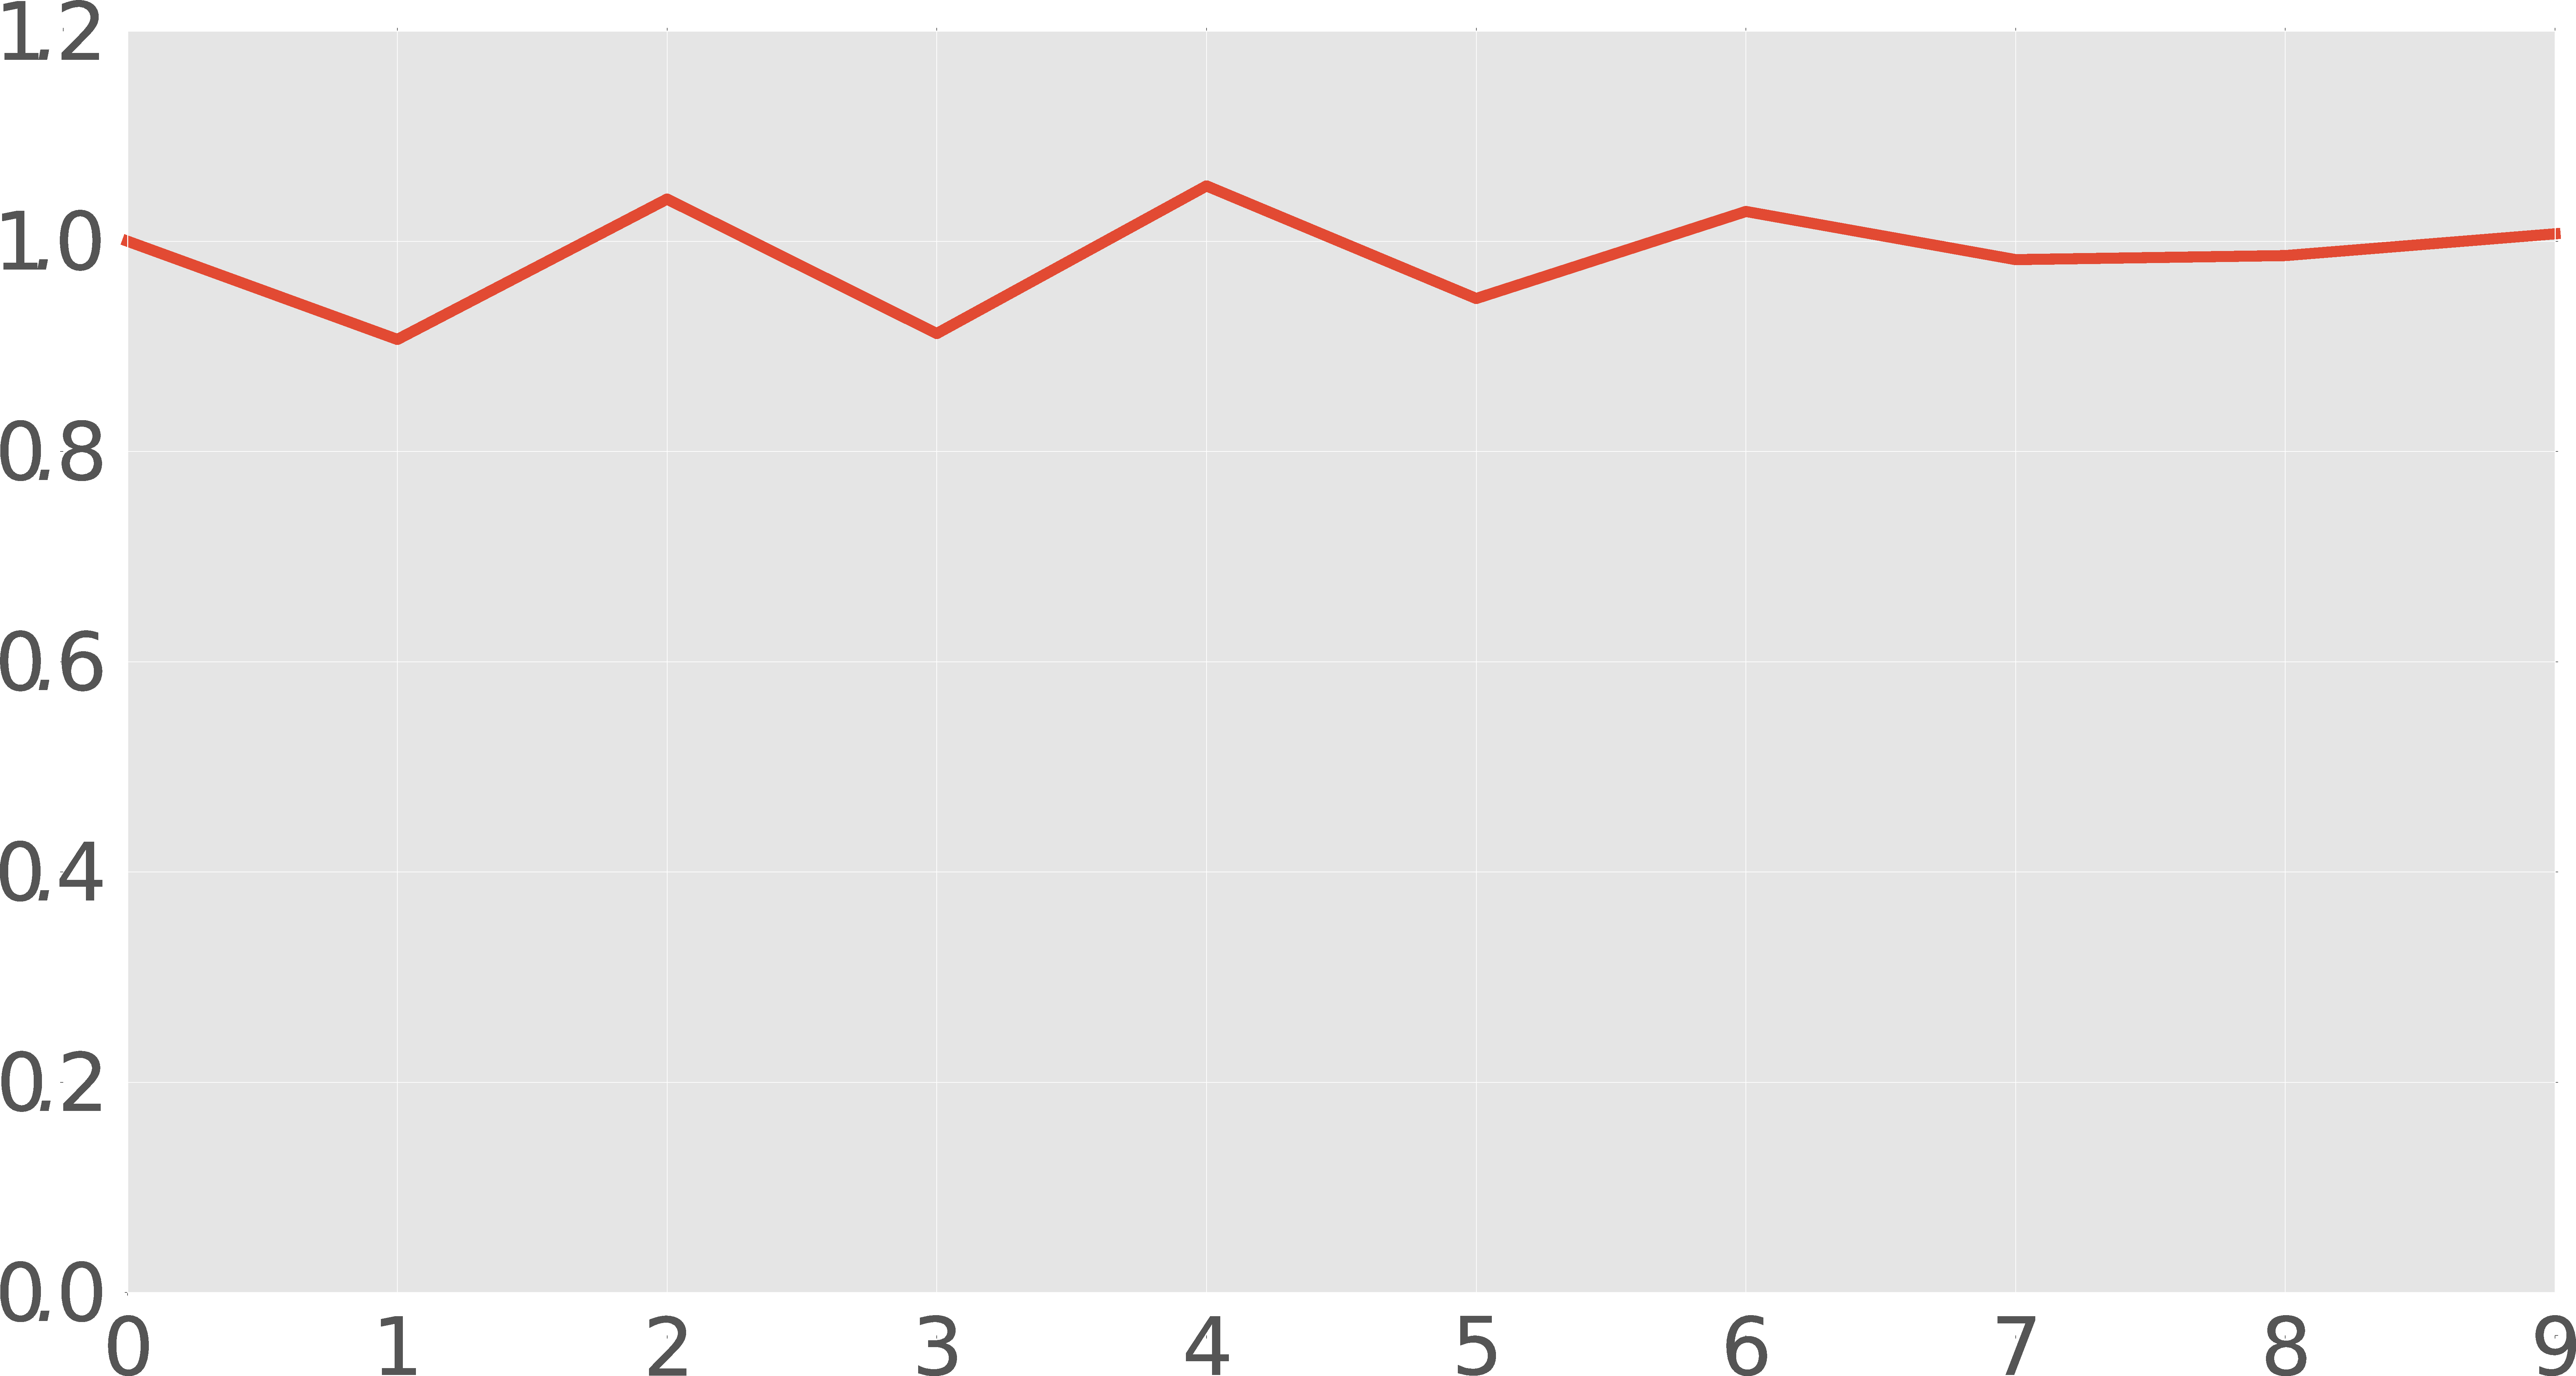
\includegraphics[width=0.8\columnwidth]{figures/reactive-transport//advection-central-scheme-oscillation} \\[5pt]
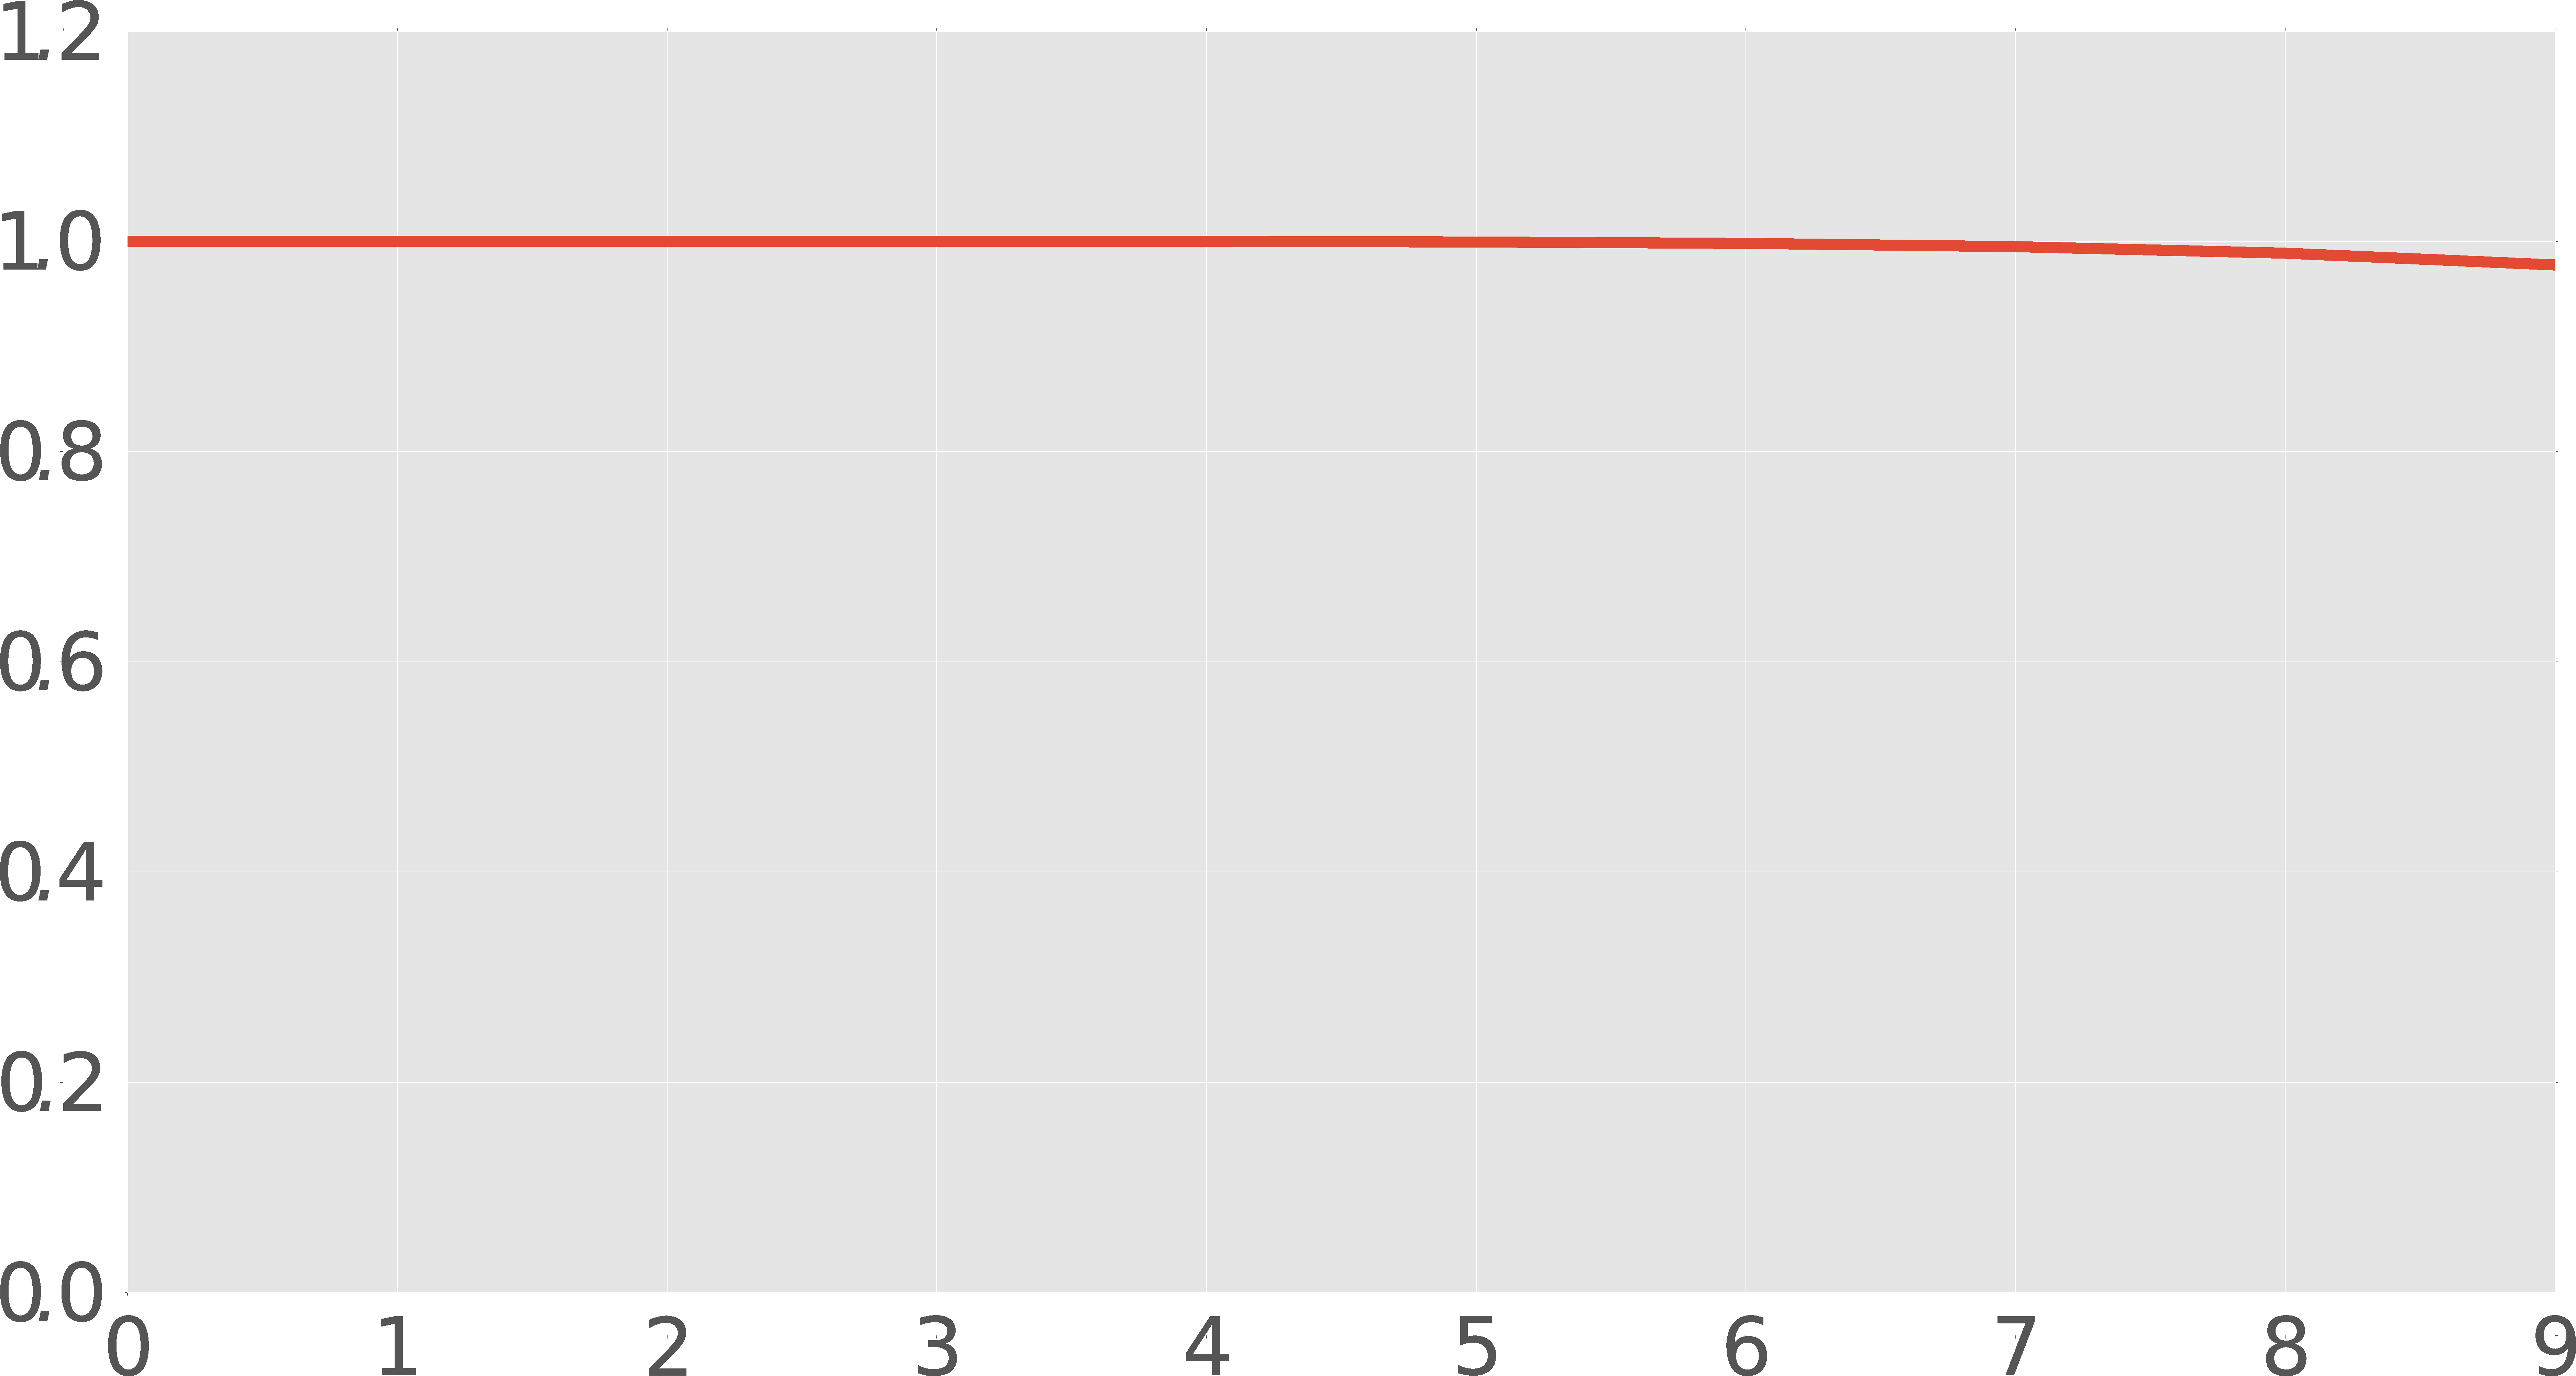
\includegraphics[width=0.8\columnwidth]{figures/reactive-transport//advection-upwind-scheme-no-oscillation}
\par\end{center}

\ecol
\end{frame}
%%
%% --------------------------------------------------------------------------------------------------------------------%
%% Discretization of the transport equations
%% --------------------------------------------------------------------------------------------------------------------%
%%
%\begin{frame}{Discretization of the transport equations}
%
%\lcol
%\begin{itemize}
%\item We'll use instead an \alert{upwind scheme}:
%\[
%\frac{\partial u}{\partial x}\approx v\left(\frac{u_{i}^{k+1}-u_{i-1}^{k+1}}{\Delta x}\right)
%\]
%to prevent this. 
%\end{itemize}
%\rcol
%\begin{center}
%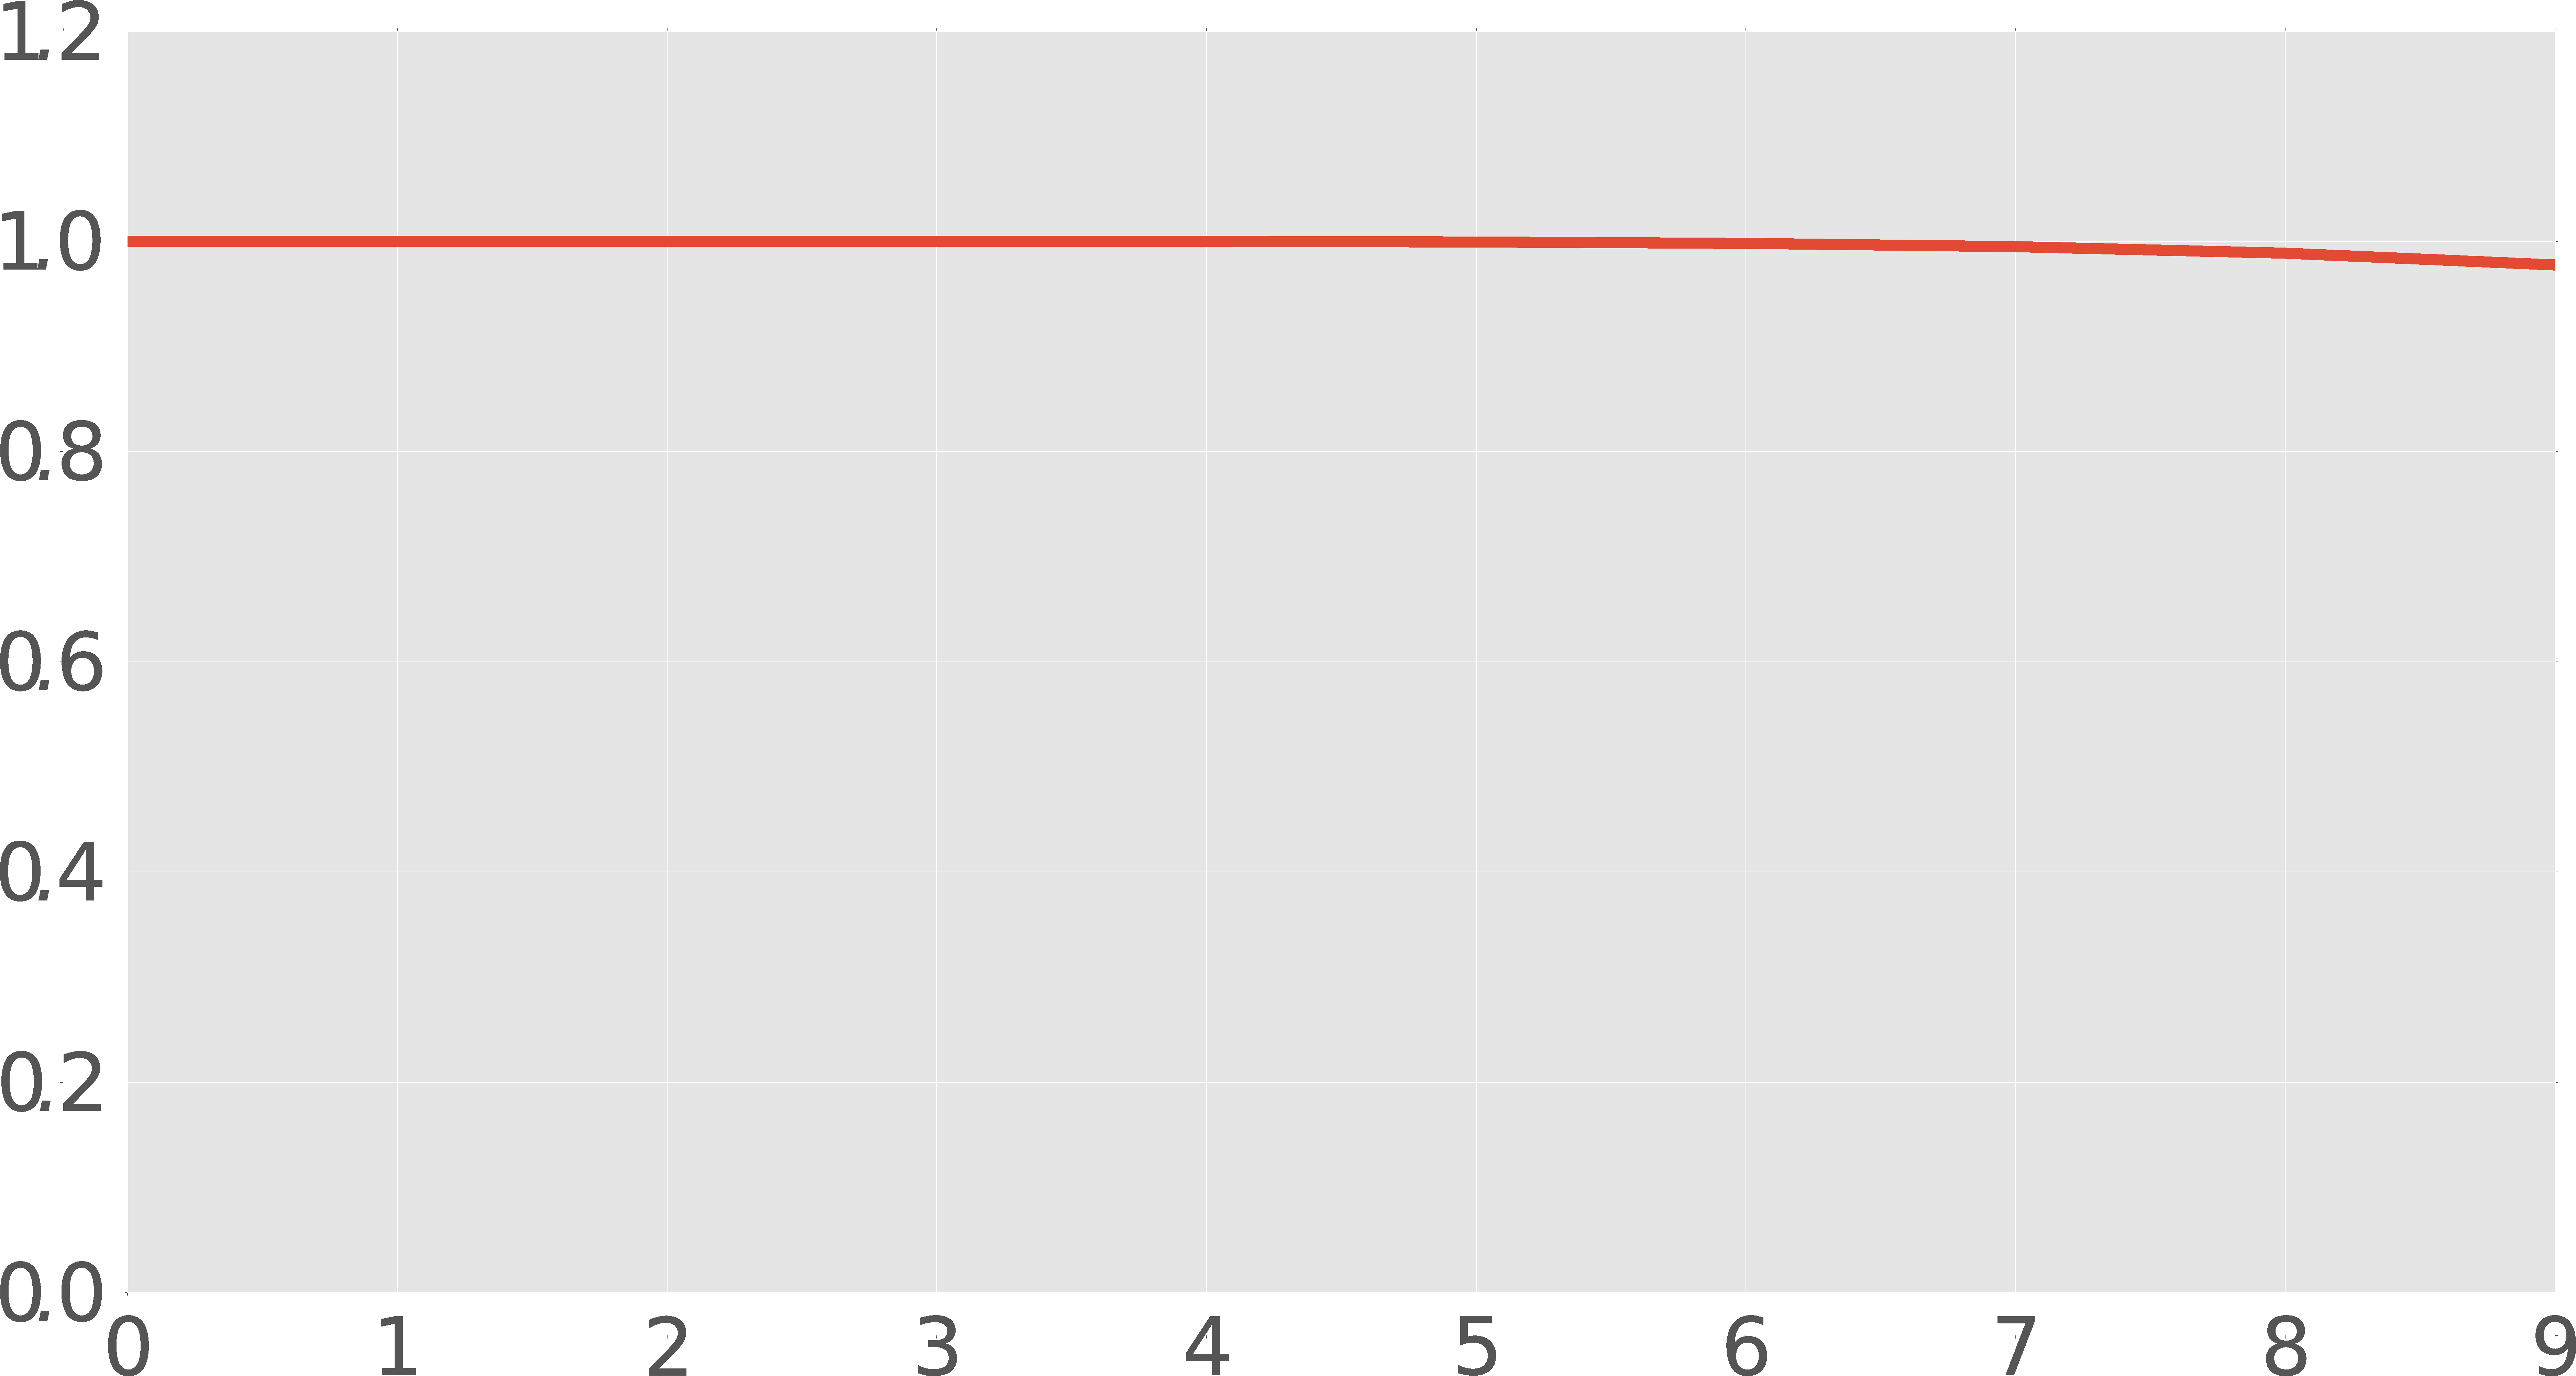
\includegraphics[width=1\columnwidth]{figures/reactive-transport//advection-upwind-scheme-no-oscillation}
%\par\end{center}
%
%\ecol
%\end{frame}
%
% --------------------------------------------------------------------------------------------------------------------%
% Numerical diffusion 
% --------------------------------------------------------------------------------------------------------------------%
%
\begin{frame}{Numerical diffusion introduced by the upwind scheme}
\begin{itemize}
\item {\bf Warning}: the upwind scheme fixes the numerical oscillation, but introduces
\alert{\bf numerical diffusion}!
\end{itemize}
\lcol
\begin{center}
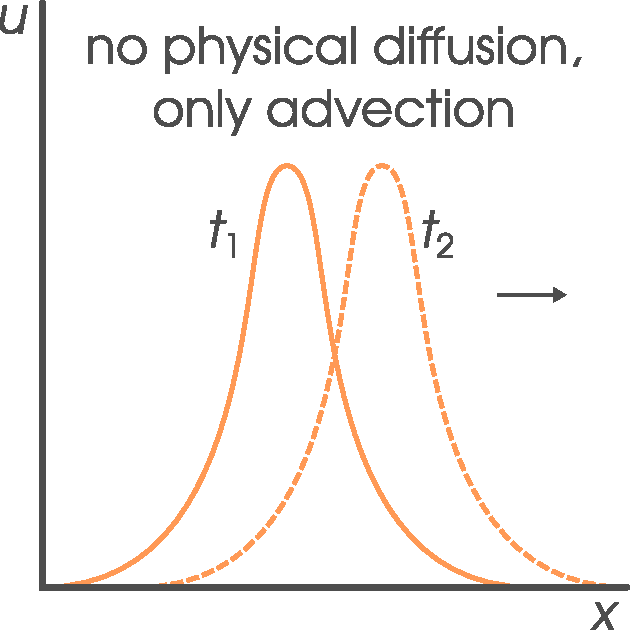
\includegraphics[height=0.6\textheight]{figures/reactive-transport//numerical-diffusion-illustration-1}
\par\end{center}

\rcol
\begin{center}
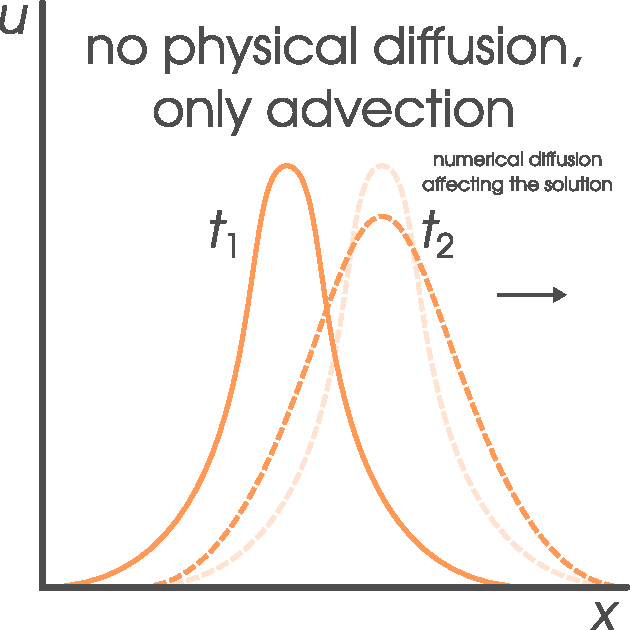
\includegraphics[height=0.6\textheight]{figures/reactive-transport//numerical-diffusion-illustration-2}
\par\end{center}

\ecol
\end{frame}
%
% --------------------------------------------------------------------------------------------------------------------%
% Discretization of the transport equations
% --------------------------------------------------------------------------------------------------------------------%
%
\begin{frame}{Discretization of transport equation: tridiagonal formulation}
\begin{itemize}
\item We write the algebraic equation
\[
\left(\frac{u_{i}^{k+1}-u_{i}^{k}}{\Delta t}\right)+v\left(\frac{u_{i}^{k+1}-u_{i-1}^{k+1}}{\Delta x}\right)-D\left(\frac{u_{i+1}^{k+1}-2u_{i}^{k+1}+u_{i-1}^{k+1}}{\Delta x^{2}}\right)=f_{i}\quad(i=1,\ldots,n-1)
\]
into the the following tridiagonal matrix form:
\[
\alert{a_{i}}\, u_{i-1}^{k+1}+
\alert{b_{i}}\, u_{i}^{k+1}+
\alert{c_{i}}\, u_{i+1}^{k+1}=
\alert{d_{i}}\, \quad(i=1,\ldots,n-1)
\]
\item \alert{\bf Tridiagonal matrix} is a band matrix that has nonzero elements on the main diagonal and first diagonal below and above it the main one.
%
% \item \alert{\bf Exercise: } Find the values of the coefficients
% $\alert{a_{i}}, \alert{b_{i}}, \alert{c_{i}},$ and $\alert{d_{i}}$.
%\item \textbf{Answer:}
\end{itemize}
%\[
%\boxed{a_{i}=-\frac{v\Delta t}{\Delta x}-\frac{D\Delta t}{\Delta x^{2}}}\quad\boxed{b_{i}=1+\frac{v\Delta t}{\Delta x}+2\frac{D\Delta t}{\Delta x^{2}}}\quad\boxed{c_{i}=-\frac{D\Delta t}{\Delta x^{2}}}\quad\boxed{d_{i}=u_{i}^{k}+\Delta tf_{i}\vphantom{\frac{D\Delta t}{\Delta x^{2}}}}
%\]

\end{frame}
%
% --------------------------------------------------------------------------------------------------------------------%
% Discretization of the transport equations
% --------------------------------------------------------------------------------------------------------------------%
%
\begin{frame}{Discretization of transport equation: internal points}

\begin{itemize}
\item For \alert{\bf every internal point} $x_{i}$, we have the system
\[
a_{i}u_{i-1}^{k+1}+b_{i}u_{i}^{k+1}+c_{i}u_{i+1}^{k+1}=d_{i}\quad(i=1,\ldots,n-1)
\]
where
\[
\boxed{a_{i}=-\frac{v\Delta t}{\Delta x}-\frac{D\Delta t}{\Delta x^{2}}}\quad\boxed{b_{i}=1+\frac{v\Delta t}{\Delta x}+2\frac{D\Delta t}{\Delta x^{2}}}\quad\boxed{c_{i}=-\frac{D\Delta t}{\Delta x^{2}}}\quad\boxed{d_{i}=u_{i}^{k}+\Delta tf_{i}\vphantom{\frac{D\Delta t}{\Delta x^{2}}}}
\]
\end{itemize}
\vskip 10pt
\begin{center}
	\includegraphics[width=0.8\textwidth]{figures/reactive-transport/finite-difference-domain-discretization}
\par\end{center}
\end{frame}
%
% --------------------------------------------------------------------------------------------------------------------%
% Discretization of the transport equations, Left boundary condition
% --------------------------------------------------------------------------------------------------------------------%
%
\begin{frame}{Discretization of transport equation: left boundary condition}
\begin{itemize}
\item On the \alert{\bf left boundary point}, $u=1$, and thus $u^{k}_{0}=u^{k+1}_{0} =1.$ 
\item \textbf{Exercises: }What are the values of $a_{0}$, $b_{0}$, $c_{0}$
and $d_{0}$ in the general equation:
\[
a_{0}u_{-1}^{k+1}+b_{0}u_{0}^{k+1}+c_{i}u_{1}^{k+1}=d_{0}?
\]
\hiddenpause
\item \textbf{Answer:} 
\[
\boxed{a_{0}=0\vphantom{\frac{D\Delta t}{\Delta x^{2}}}}\quad\boxed{b_{0}=1\vphantom{\frac{D\Delta t}{\Delta x^{2}}}}\quad\boxed{c_{0}=0\vphantom{\frac{D\Delta t}{\Delta x^{2}}}}\quad\boxed{d_{0}=1\vphantom{\frac{D\Delta t}{\Delta x^{2}}}}
\]
\end{itemize}
\end{frame}
%
% --------------------------------------------------------------------------------------------------------------------%
% Discretization of the transport equations, Right boundary condition
% --------------------------------------------------------------------------------------------------------------------%
%
\begin{frame}{Discretization of transport equation: right boundary condition}

%\lcol
\begin{itemize}
\item On the \alert{\bf right boundary point}, we use the following finite difference representation for the \textbf{advection} and  \textbf{diffusion terms}:
%\[
%\left(v\frac{\partial u}{\partial x}\right)_{n}^{k+1} \quad \mbox{and} \quad
%\left(D\frac{\partial^{2}u}{\partial x^{2}}\right)_{n}^{k+1}, \quad \mbox{resp.}
%\]
%\item We use the following discretizations:
\[
\left(v\frac{\partial u}{\partial x}\right)_{n}^{k+1}=v\frac{u_{n}^{k+1}-u_{n-1}^{k+1}}{\Delta x} 
\quad \mbox{and} \quad
\left(D\frac{\partial^{2}u}{\partial x^{2}}\right)_{n}^{k+1}=0.
\]
\item Then, the algebraic equation reads as
\[
a_{n}u_{n-1} + b_{n}u_{n} + c_{n}u_{n+1} =d_{n}
\]
with
\[
\boxed{a_{n}=-\frac{v\Delta t}{\Delta x}}\quad\boxed{b_{n}=1+\frac{v\Delta t}{\Delta x}}\quad\boxed{c_{n}=0\vphantom{\frac{D\Delta t}{\Delta x^{2}}}}\quad\boxed{d_{n}=u_{n}^{k}+\Delta tf_{n-1}\vphantom{\frac{D\Delta t}{\Delta x^{2}}}}.
\]
\end{itemize}
%\ecol
\end{frame}
%%
%% --------------------------------------------------------------------------------------------------------------------%
%% Discretization of the transport equations, Right boundary condition
%% --------------------------------------------------------------------------------------------------------------------%
%%
%\begin{frame}{Discretization of the transport equations: Right boundary condition}
%
%\scriptsize
%
%\lcol
%\begin{itemize}
%\item The discretization of:
%\[
%\frac{\partial u}{\partial t}+v\frac{\partial u}{\partial x}-D\frac{\partial^{2}u}{\partial x}=f
%\]
%results in: 
%\[
%\left(\frac{u_{i}^{k+1}-u_{i}^{k}}{\Delta t}\right)+v\left(\frac{u_{i+1}^{k+1}-u_{i-1}^{k+1}}{2\Delta x}\right)-
%%D\left(\frac{u_{i+1}^{k+1}-2u_{i}+u_{i-1}^{k+1}}{\Delta x^{2}}\right)=f_{i}
%\]
%for interior nodes $i=1,\ldots,n-1$. 
%\item \textbf{Exercise:} Find the values of $a_{n}$, $b_{n}$, $c_{n}$
%and $d_{n}$ in the general algebraic equation:
%\[
%a_{i}u_{i-1}^{k+1}+b_{i}u_{i}^{k+1}+c_{i}u_{i+1}^{k+1}=d_{i}\quad(i=n)?
%\]
%\end{itemize}
%\rcol
%\begin{itemize}
%\item Consider:
%\[
%\left(v\frac{\partial u}{\partial x}\right)_{n}^{k+1}=v\frac{u_{n}^{k+1}-u_{n-1}^{k+1}}{\Delta x}
%\qquad\text{and}\qquad
%\left(D\frac{\partial^{2}u}{\partial x^{2}}\right)_{n}^{k+1}=0.
%\]
%\hiddenpause
%\item \textbf{Answer:} The algebraic equation is:
%\[
%\left(-\frac{v\Delta t}{\Delta x}\right)u_{n-1}^{k+1}+\left(1+\frac{v\Delta t}{\Delta x}\right)u_{n}^{k+1}=u_{n}^{k}+\Delta tf_{n-1},
%\]
%and thus:
%\[
%\boxed{a_{n}=-\frac{v\Delta t}{\Delta x}}\quad\boxed{b_{n}=1+\frac{v\Delta t}{\Delta x}}\quad\boxed{c_{n}=0\vphantom{\frac{D\Delta t}{\Delta x^{2}}}}\quad\boxed{d_{n}=u_{n}^{k}+\Delta tf_{n-1}\vphantom{\frac{D\Delta t}{\Delta x^{2}}}}
%\]
%\end{itemize}
%\ecol
%\end{frame}
%
% --------------------------------------------------------------------------------------------------------------------%
% Solving a tridiagonal matrix equation
% --------------------------------------------------------------------------------------------------------------------%
%
\begin{frame}{Solving a tridiagonal matrix equation}
\vskip -15pt
%
\begin{alignat*}{2}
b_{0}u_{0}+c_{0}u_{1} & =d_{0} &  & (i=0)\\
a_{i}u_{i-1}^{k+1}+b_{i}u_{i}^{k+1}+c_{i}u_{i+1}^{k+1} & =d_{i} & \qquad & (i=1,\ldots,n-1)\\
a_{n}u_{n-1}+b_{n}u_{n} & =d_{n} &  & (i=n)
\end{alignat*}
%
or
%
\[
\begin{bmatrix}b_{0} & c_{0}\\
a_{1} & b_{1} & c_{1}\\
 & a_{2} & b_{2} & c_{2}\\
 %&  & a_{3} & b_{3} & \cdot\\
 &  &  \ddots & \ddots & \ddots & \\
 &  &  & a_{n-1} & b_{n-1} & c_{n-1}\\
 &  &  &  & a_{n} & b_{n}
\end{bmatrix}\begin{bmatrix}u_{0}\\
u_{1}\\
u_{2}\\
\cdot\\
u_{n-1} \\
u_{n}
\end{bmatrix}=\begin{bmatrix}d_{0}\\
d_{1}\\
d_{2}\\
\cdot\\
d_{n-1} \\
d_{n}
\end{bmatrix}
\]
\begin{itemize}
	\item This special linear system can be solved using the \alert{\bf Thomas matrix algorithm}.
	\item The algorithm is stable for the \alert{\bf diagonally dominant} or \alert{\bf  positive definite} matrices.
\end{itemize}

\end{frame}
%
% --------------------------------------------------------------------------------------------------------------------%
% Thomas algorithm in Pythonx
% --------------------------------------------------------------------------------------------------------------------%
%
\begin{frame}[fragile]{Thomas algorithm in Python}

\begin{lstlisting}[language=Python, caption=Thomas algorithm for tridiagonal matrices]
	def thomas(a, b, c, d):
		# Size of the matrix
		n = len(d)
		# Calculation of new coeffitients 
		c[0] /= b[0]
		for i in range(1, n - 1):
			c[i] /= b[i] - a[i]*c[i - 1]
			d[0] /= b[0]
		# The forward sweep 
		for i in range(1, n):
			d[i] = (d[i] - a[i]*d[i - 1])/(b[i] - a[i]*c[i - 1])
		x = d
		# The backward sweep 
		for i in reversed(range(0, n - 1)):
			x[i] -= c[i]*x[i + 1]
		return x
\end{lstlisting}

\end{frame}
%
% --------------------------------------------------------------------------------------------------------------------%
% Transport step in Python
% --------------------------------------------------------------------------------------------------------------------%
%
\begin{frame}[fragile]{Transport step in Python}

\begin{lstlisting}[language=Python, caption=Transport step in Pythons]
	beta, alpha = v * dt / dx,  D * dt / dx**2
	def transport(u):
		# Coefficients a, b, c
		a.fill(-beta - alpha)
		b.fill(1 + beta + 2*alpha)
		c.fill(-alpha)
		# Coefficients a, b, c on the left boundary node
		a[0] = 0.0
		b[0] = 1.0
		c[0] = 0.0
		# Coefficients a, b, c on the right boundary node
		a[-1] = -beta
		b[-1] = 1 + beta
		c[-1] = 0.0
		# Dirichlet boundary condition for u on the left boundary node
		u[0] = ul
		# Solve the tridiagonal matrix equation
		thomas(a, b, c, u)
\end{lstlisting}

\end{frame}
%
% --------------------------------------------------------------------------------------------------------------------%
% Reactive transport in a single fluid phase
% --------------------------------------------------------------------------------------------------------------------%
%
\subsection{Reactive transport in a single fluid phase}
\begin{frame}{Reactive transport in a single fluid phase}
\begin{itemize}
\item Consider a \alert{\bf single fluid phase} with N chemical species.
\item Each species is transported according to the following N \alert{\bf reactive transport equations}
\[
\frac{\partial n_{i}}{\partial t}+\nabla\cdot(n_{i}\boldsymbol{v}-D\nabla n_{i})=r_{i}\qquad(i=1,\ldots,\mathsf{N}),
\]
where
\begin{itemize}
\item $n_{i}$ is the \alert{concentration} of species $i$ (in mol/m$^{3}$);
\item $\boldsymbol{v}$ is the \alert{fluid velocity}
(in m/s);
\item $D$ is the \alert{diffusion coefficient} of the species (in m$^{2}$/s);
\item $r_{i}$ is the \alert{rate of production\slash consumption} of species
$i$ (in mol/(m$^{3}\cdot$s)). 
\end{itemize}
\end{itemize}
\end{frame}
%
% --------------------------------------------------------------------------------------------------------------------%
% Local chemical equilibrium assumption
% --------------------------------------------------------------------------------------------------------------------%
%
\begin{frame}[<+->]{Local chemical equilibrium assumption \, i}
\begin{itemize}
\item The \alert{\bf rates of transport} (advection and diffusion) can sometimes
be {\bf considerably slower }than the \alert{\bf rates of chemical reactions}.
\item \alert{\bf Advection flux rates} are $n_{i}v\approx10^{-5}\;\mathsf{mol/(m^{2}\cdot s)}$,
considering $v\approx1\;\mathsf{m/day}$.
\item \alert{\bf Diffusion flux rates} are $-D\nabla n_{i}\approx10^{-9}\;\mathsf{mol/(m^{2}\cdot s)}$,
considering $D\approx10^{-9}\;\mathsf{m^{2}/s}$.
\item \alert{\bf Rates of aqueous reactions} are several orders of magnitude
higher, e.g., the reaction
\[
\mathsf{H^{+}+OH^{-}\rightarrow H_{2}O(aq)}
\]
has a rate of $r_{i}\approx10^{11}\;\mathsf{mol/(m^3\cdot s)}$. 
\item Many aqueous reactions {\bf equilibrate} in the order of microseconds
to few seconds!
\end{itemize}
\end{frame}
%
% --------------------------------------------------------------------------------------------------------------------%
% Local chemical equilibrium assumption, ii
% --------------------------------------------------------------------------------------------------------------------%
%
\begin{frame}{Local chemical equilibrium assumption \, ii}
\begin{itemize}
\item If chemical reactions proceed at a rate much faster than transport
rates, we can assume the species react \textbf{instantaneously to
equilibrium}.
\pause
\item Then, these chemical species are assumed to be in \alert{\bf local chemical equilibrium}
(i.e., at every point in space, they are in chemical equilibrium).
\begin{itemize}
\item As soon as the chemical species are perturbed due to advection and
diffusion, they instantaneously react to achieve a new state of equilibrium.
\item For example, as water flows through a reactive porous rock, the fluid gets immediately saturated with the rock minerals.
\end{itemize}
\pause
\item We will see that, at every time step, {a chemical equilibrium calculation	is needed at every node}, which could be computationally demanding.
%
\vskip 20pt
\begin{figure}
\centering{}\includegraphics[width=0.6\textwidth]{figures/reactive-transport//finite-difference-domain-discretization}
\end{figure}
\end{itemize}
\end{frame}
%
% --------------------------------------------------------------------------------------------------------------------%
% Simplifying the reactive transport equations 
% --------------------------------------------------------------------------------------------------------------------%
%
\begin{frame}[<+->]{Simplifying the reactive transport equations}
\begin{itemize}
\item We will now simplify the reactive transport equations
\[
\frac{\partial n_{i}}{\partial t}+\nabla\cdot(n_{i}\boldsymbol{v}-D\nabla n_{i})=r_{i}\qquad(i=1,\ldots,\mathsf{N}),
\]
using the assumption that the species are in \alert{local chemical equilibrium}. 
\item Since the species are in equilibrium at all times, the reaction rates
$r_{i}$ \alert{depend on the rates of transport} and \alert{cannot be calculated in advance}.
\item However, there is a way to \textbf{eliminate} them and \textbf{drastically
reduce the number of transport equations} to solve!
\end{itemize}
\end{frame}
%
% --------------------------------------------------------------------------------------------------------------------%
% Simplifying the reactive transport equations 
% --------------------------------------------------------------------------------------------------------------------%
%
\begin{frame}{Things we need in the simplification}
\begin{itemize}

\item Contribution of each species to the \alert{\bf concentration of element $j$}:
\[
b_j = \sum_{i=1}^{\mathrm{N}}A_{ji}n_{i}.
\]
%
\item \alert{\bf Rate of production of every chemical
element} and according to {\bf the mass conservation condition for the elements}:
%
\[
\sum_{i=1}^{\mathrm{N}}A_{ji}r_{i}=0.
\]
\end{itemize}
\end{frame}
%
% --------------------------------------------------------------------------------------------------------------------%
% Simplifying the reactive transport equations 
% --------------------------------------------------------------------------------------------------------------------%
%
%\begin{frame}{Simplifying the reactive transport equations }
%\begin{columns}[t]
%
%\column{0.5\textwidth}
%\begin{itemize}
%\item \textbf{Question:} If the concentration of element $j$ is given by:
%\[
%\sum_{i=1}^{\mathrm{N}}A_{ji}n_{i}=\begin{pmatrix}\text{concentration}\\
%\text{of element \ensuremath{j}}
%\end{pmatrix}=b_{j},
%\]
%what is the result of this sum:
%\[
%\sum_{i=1}^{\mathrm{N}}A_{ji}r_{i}=\;?
%\]
%\hiddenpause
%\end{itemize}
%
%\column{0.5\textwidth}
%\begin{itemize}
%\item \textbf{Answer:} This sum computes the \alert{rate of production of element $j$}:
%\[
%\sum_{i=1}^{\mathrm{N}}A_{ji}r_{i}=\begin{pmatrix}\text{rate of production}\\
%\text{of element \ensuremath{j}}
%\end{pmatrix}
%\]
%\hiddenpause\textbf{ }
%\item \textbf{Question:} What is the rate of production of every chemical
%element?
%\end{itemize}
%\end{columns}
%
%\end{frame}
%%
%% --------------------------------------------------------------------------------------------------------------------%
%% Simplifying the reactive transport equations 
%% --------------------------------------------------------------------------------------------------------------------%
%%
%\begin{frame}{Simplifying the reactive transport equations }
%\begin{itemize}
%\item We have now determined that:
%\[
%\sum_{i=1}^{\mathrm{N}}A_{ji}r_{i}=0.
%\]
%\item \textbf{Question:} How can we use this to eliminate the reaction rates
%$r_{i}$ in the reactive transport equations for the chemical species:
%\[
%\frac{\partial n_{i}}{\partial t}+\nabla\cdot(n_{i}\boldsymbol{v}-D\nabla n_{i})=r_{i}\qquad(i=1,\ldots,\mathsf{N})?
%\]
%\end{itemize}
%\end{frame}
%%
%% --------------------------------------------------------------------------------------------------------------------%
%% Reactive transport equations in terms of element concentrations
%% --------------------------------------------------------------------------------------------------------------------%
%%
%\begin{frame}{Reactive transport equations in terms of element concentrations}
%
%\small
%\begin{itemize}
%\item \alert{\textbf{Exercise:}} Use 
%\[
%\sum_{i=1}^{\mathrm{N}}A_{ji}n_{i}=b_{j}\qquad\text{and}\qquad\sum_{i=1}^{\mathrm{N}}A_{ji}r_{i}=0
%\]
%to simplify the \textbf{N transport equations} (in terms of species
%concentrations $n_{i}$), i.e., 
%\[
%\frac{\partial n_{i}}{\partial t}+\nabla\cdot(n_{i}\boldsymbol{v}-D\nabla n_{i})=r_{i}\qquad(i=1,\ldots,\mathsf{N})
%\]
%into \textbf{E transport equations} in terms of element concentrations
%$b_{j}$. 
%\hiddenpause
%\item \textbf{Answer:}
%\[
%\frac{\partial b_{j}}{\partial t}-\nabla\cdot(b_{j}\boldsymbol{v}-D\nabla b_{j})=0\qquad(j=1,\ldots,\mathsf{E}).
%\]
%\end{itemize}
%\end{frame}
%%
%% --------------------------------------------------------------------------------------------------------------------%
%% Transport step followed by equilibrium step
%% --------------------------------------------------------------------------------------------------------------------%
%%
%\begin{frame}{Transport step followed by equilibrium step}
%The \alert{\bf reactive transport calculation step} for aqueous phase only:
%\begin{itemize}
%\item {\bf Update the concentrations of the elements} $b_{j}^{k+1}$, using the finite difference discretization (at teach time step and in every mesh node)
%\[
%\frac{b^{k+1}_{j} - b^k_{j}}{dt}+\nabla\cdot(b^{k+1}_{j}\boldsymbol{v}-D\nabla b^{k+1}_{j})=0\qquad(j=1,\ldots,\mathsf{E}).
%\]
%%
%%
%%\item \textbf{Question:} This transport step involves no chemical reaction
%%calculations. What should we compute next with the updated $b_{\mathrm{H}}^{k+1}$,
%%$b_{\mathrm{O}}^{k+1}$, $b_{\mathrm{C}}^{k+1}$, $b_{\mathrm{Ca}}^{k+1}$,
%%etc.? \hiddenpause
%\item {\bf Update the species concentrations} $n=[n_{e}, n_k]$, $n_e \in \mathbb{R}^{N_e}$ and $n_k \in \mathbb{R}^{N_k}$, calculated at every node %, using a chemical equilibrium calculation:
%%
%\begin{alignat*}{4}
%	\frac{\mathrm{d}b_{e}}{\mathrm{d}t} & = f_e(n_e)& \qquad & t>0, & \quad  \quad b_{e}=b^{\circ}_{e} = b^{k+1}_{j} & \qquad & t=0,\label{eq:full-kinetics}\\
%	\frac{\mathrm{d}n_{k}}{\mathrm{d}t} & = f_k(n_k) &  & t>0, & \quad n_{k}=n_{k}^{\circ} \quad \quad \quad &  & t=0,\nonumber \\
%	n_{e} & =\varphi(T,P,b_{e}) &  & t>0. & &  &\nonumber 
%\end{alignat*}
%%\[
%%\min_{n}G(n)\qquad\text{subject to}\qquad An=b\quad\text{and}\quad n\geq0.
%%\]
%\end{itemize}
%\end{frame}
%
% --------------------------------------------------------------------------------------------------------------------%
% Reactive transport combined with aqueous–mineral reactions --------------------------------------------------------------------------------------------------------------------%
%
\begin{frame}[<+->]{Reactive transport combined with aqueous-mineral reactions}
\begin{itemize}
\item We start from the equation for a \alert{\bf single fluid phase}
\[
\frac{\partial n_{i}}{\partial t}+\nabla\cdot(n_{i}\boldsymbol{v}-D\nabla n_{i})=r_{i}\qquad(i=1,\ldots,\mathsf{N}).
\]
\item If \alert{\bf mineral species} are present, they are \alert{\bf immobile}. 
\item We \alert{\bf partition the species to fluid and solid species} with corresponding amount of elements $b^{\rm f}$ and $b^{\rm s}$, such that the {\bf reactions that occur among
aqueous and mineral species} are governed as follows:
%
\begin{alignat*}{2}
\frac{\partial n^{\rm f}_{i}}{\partial t}+\nabla\cdot(n^{\rm f}_{i}\boldsymbol{v}-D\nabla n^{\rm f}_{i}) & =r^{\rm f}_{i} & \qquad & (i=1,\ldots,\mathsf{N^{\rm f}}),\\
\frac{\partial n^{\rm s}_{i}}{\partial t} & =r^{\rm s}_{i} &  & (i=1,\ldots,\mathsf{N^{\rm s}}),
\end{alignat*}
%
where superscript $\mathsf{s}$ refers to solid, and $\mathsf{f}$
to fluid.
\end{itemize}
\end{frame}
%
\begin{frame}{Reactive transport equations in terms of element concentrations}

\alert{\textbf{Exercise:}} Using the fact that
\[
b_{j}=b_{j}^{\mathsf{f}}+b_{j}^{\mathsf{s}}=\sum_{i=1}^{\mathsf{N^{f}}}A_{ji}n_{i}+\sum_{i=1}^{\mathsf{N^{s}}}A_{ji}n_{i}=\sum_{i=1}^{\mathsf{N}}A_{ji}n_{i}
\]
and
\[
\sum_{i=1}^{\mathsf{N}}A_{ji}r_{i}=0,
\]
%
derive
\[
\frac{\partial b_{j}^{\mathsf{s}}}{\partial t}+\frac{\partial b_{j}^{\mathsf{f}}}{\partial t}+\nabla\cdot(b_{j}^{\mathsf{f}}\boldsymbol{v}-D\nabla b_{j}^{\mathsf{f}})=0\qquad(j=1,\ldots,\mathsf{E}).
\]

\end{frame}
%
% --------------------------------------------------------------------------------------------------------------------%
% Reactive transport equations in terms of element concentrations --------------------------------------------------------------------------------------------------------------------%
%
\begin{frame}{Reactive transport equations in terms of element concentrations}
	\small 
\alert{\bf To solve} \\[-10pt]
\[
\frac{\partial b_{j}^{\mathsf{s}}}{\partial t}+\frac{\partial b_{j}^{\mathsf{f}}}{\partial t}+\nabla\cdot(b_{j}^{\mathsf{f}}\boldsymbol{v}-D\nabla b_{j}^{\mathsf{f}})=0\qquad(j=1,\ldots,\mathsf{E}),
\]
we use the following \alert{\bf operator splitting} scheme: 
\small
\begin{itemize}
	%
	\item \textbf{Step 1:} Ignore the changes in $b_{j}^{\mathsf{s}}$ and
	calculate $b_{j}^{\mathsf{f}}$ in every node using
	\[
	\frac{\partial b_{j}^{\mathsf{f}}}{\partial t}+\nabla\cdot(b_{j}^{\mathsf{f}}\boldsymbol{v}-D\nabla b_{j}^{\mathsf{f}})=0\qquad(j=1,\ldots,\mathsf{E}).
	\]
	\item \textbf{Step 2: }Use the updated amounts of elements in the fluid
	with the elements in the solid to calculate {\bf the amount of elements $b_{j}=b_{j}^{\mathsf{s}}+b_{j}^{\mathsf{f}}.$}
%	\[
%	b_{j}=b_{j}^{\mathsf{s}}+b_{j}^{\mathsf{f}}.
%	\]
%	\item \textbf{Step 3:} Use the updated values of $b_{j}$ to calculate {\bf the
%	equilibrium concentrations of the species $n_{i}$}.
\end{itemize}
%
\pause
\vskip 5pt
\alert{\bf Update the species concentrations} $n=[n_{e}, n_k]$, $n_e \in \mathbb{R}^{N_e}$ and $n_k \in \mathbb{R}^{N_k}$, calculated at every node %, using a chemical equilibrium calculation:
%
\begin{alignat*}{4}
	\frac{\mathrm{d}b_{e}}{\mathrm{d}t} & = f_e(n_e)& \qquad & t>0, & \quad  b_{e}=b^{\circ}_{e} = b_{j} & \qquad & t=0,\label{eq:full-kinetics}\\[-5pt]
	\frac{\mathrm{d}n_{k}}{\mathrm{d}t} & = f_k(n_k) &  & t>0, & \quad \quad  n_{k}=n_{k}^{\circ} \quad \quad \quad &  & t=0,\nonumber \\[-5pt]
	n_{e} & =\varphi(T,P,b_{e}) &  & t>0. & &  &\nonumber 
\end{alignat*}
%\[
%\min_{n}G(n)\qquad\text{subject to}\qquad An=b\quad\text{and}\quad n\geq0.
%\]
\end{frame}
%
% --------------------------------------------------------------------------------------------------------------------%
% Example, Kinetic dissolution of carbonates
% --------------------------------------------------------------------------------------------------------------------%
%
\subsection{Example of reactive transport modeling of microbial souring}
%
\begin{frame}
	\Wider{
		\begin{figure}[!t]
		\centering
		\vskip 10pt
		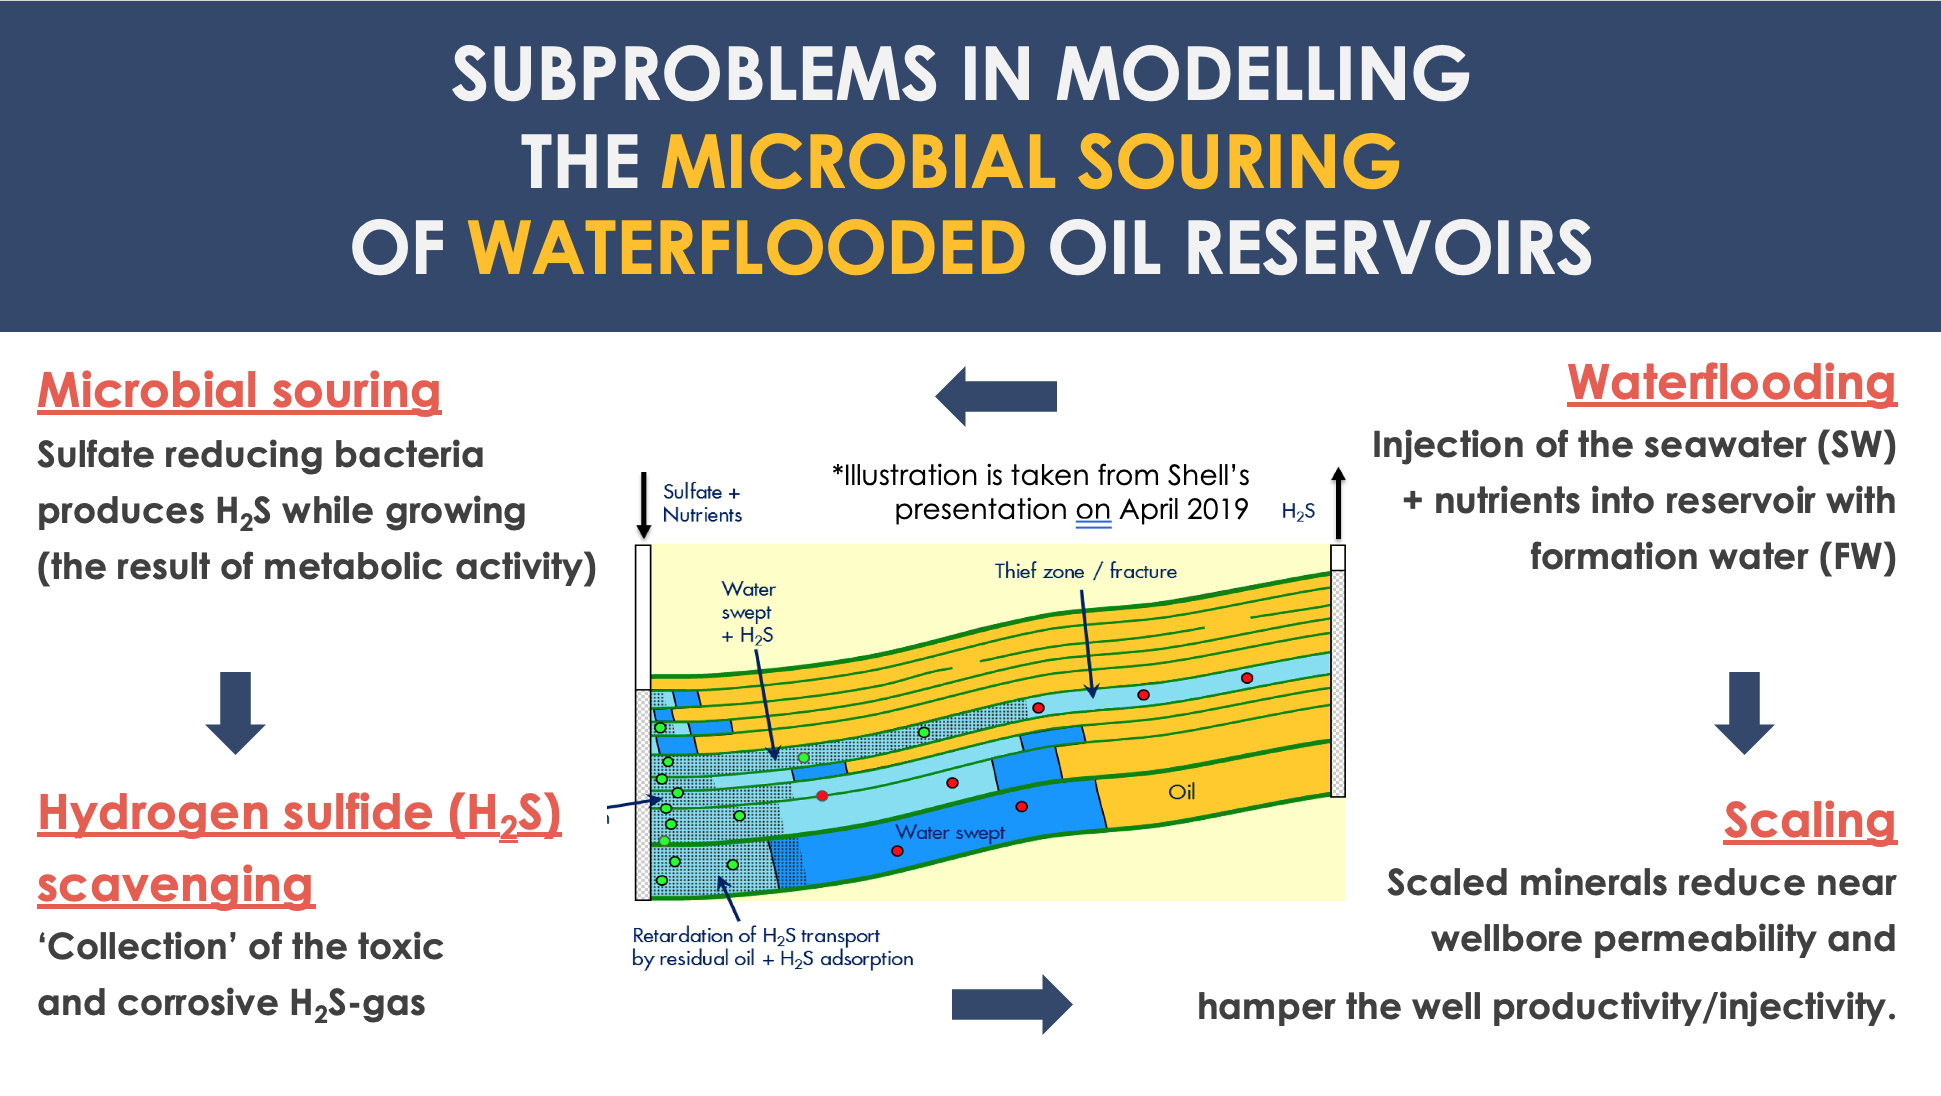
\includegraphics[width=1.0\textwidth]{figures/reactive-transport/subproblems-souring.png}
		%		%
		\end{figure}
	}
\end{frame}
%
%
\begin{frame}
	\Wider{
		\begin{figure}[!t]
			\centering
			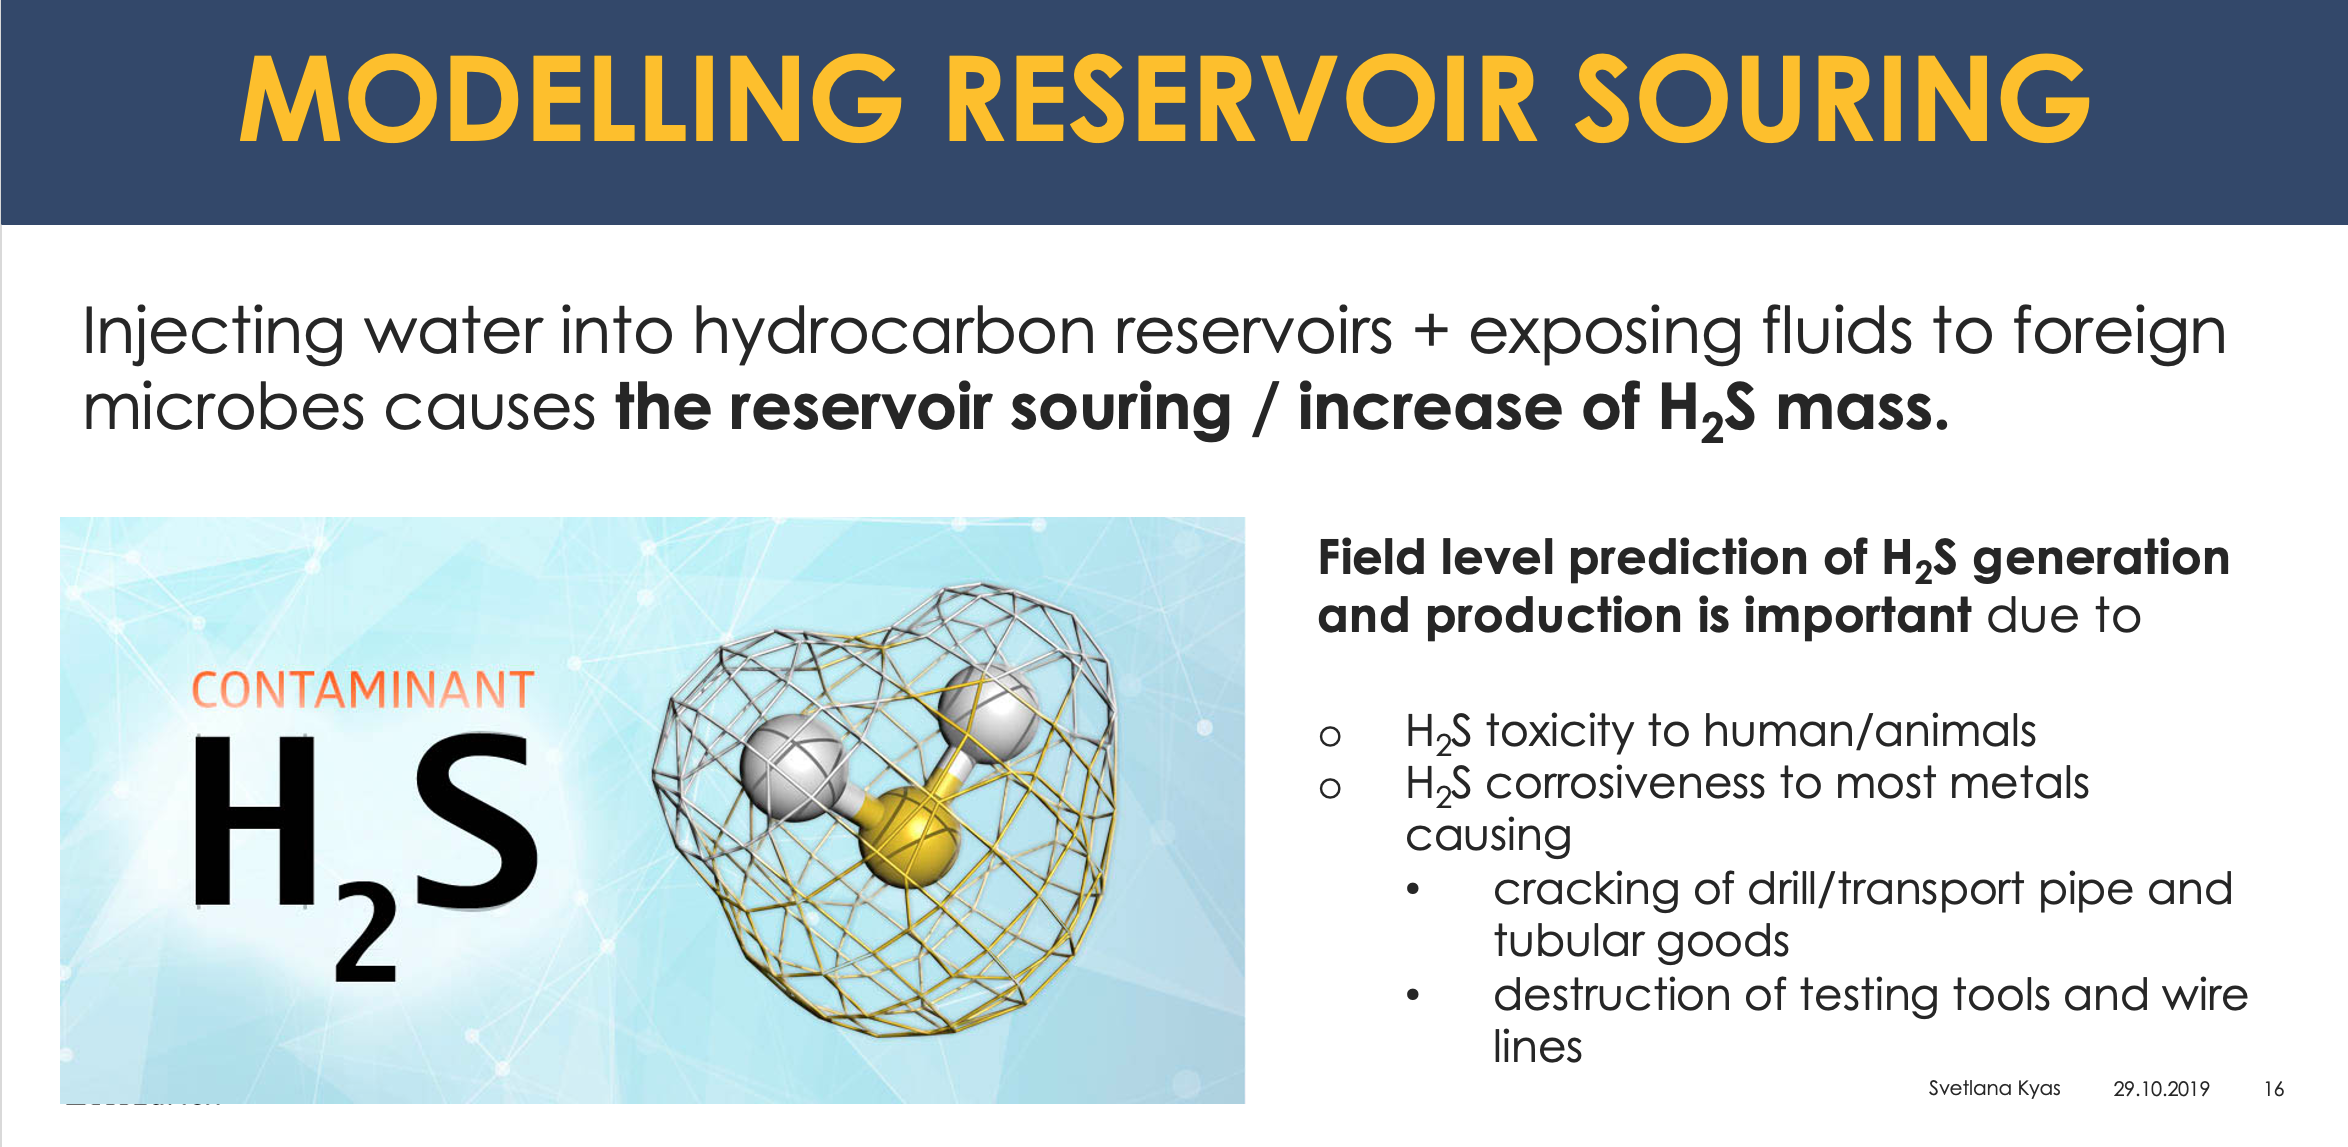
\includegraphics[width=1.0\textwidth]{figures/reactive-transport/modelling-reserviour-souring.png}
			%		%
		\end{figure}
	}
\end{frame}
%
\begin{frame}
	\Wider{
		\vskip 10pt
		\begin{figure}[!t]
		\centering
		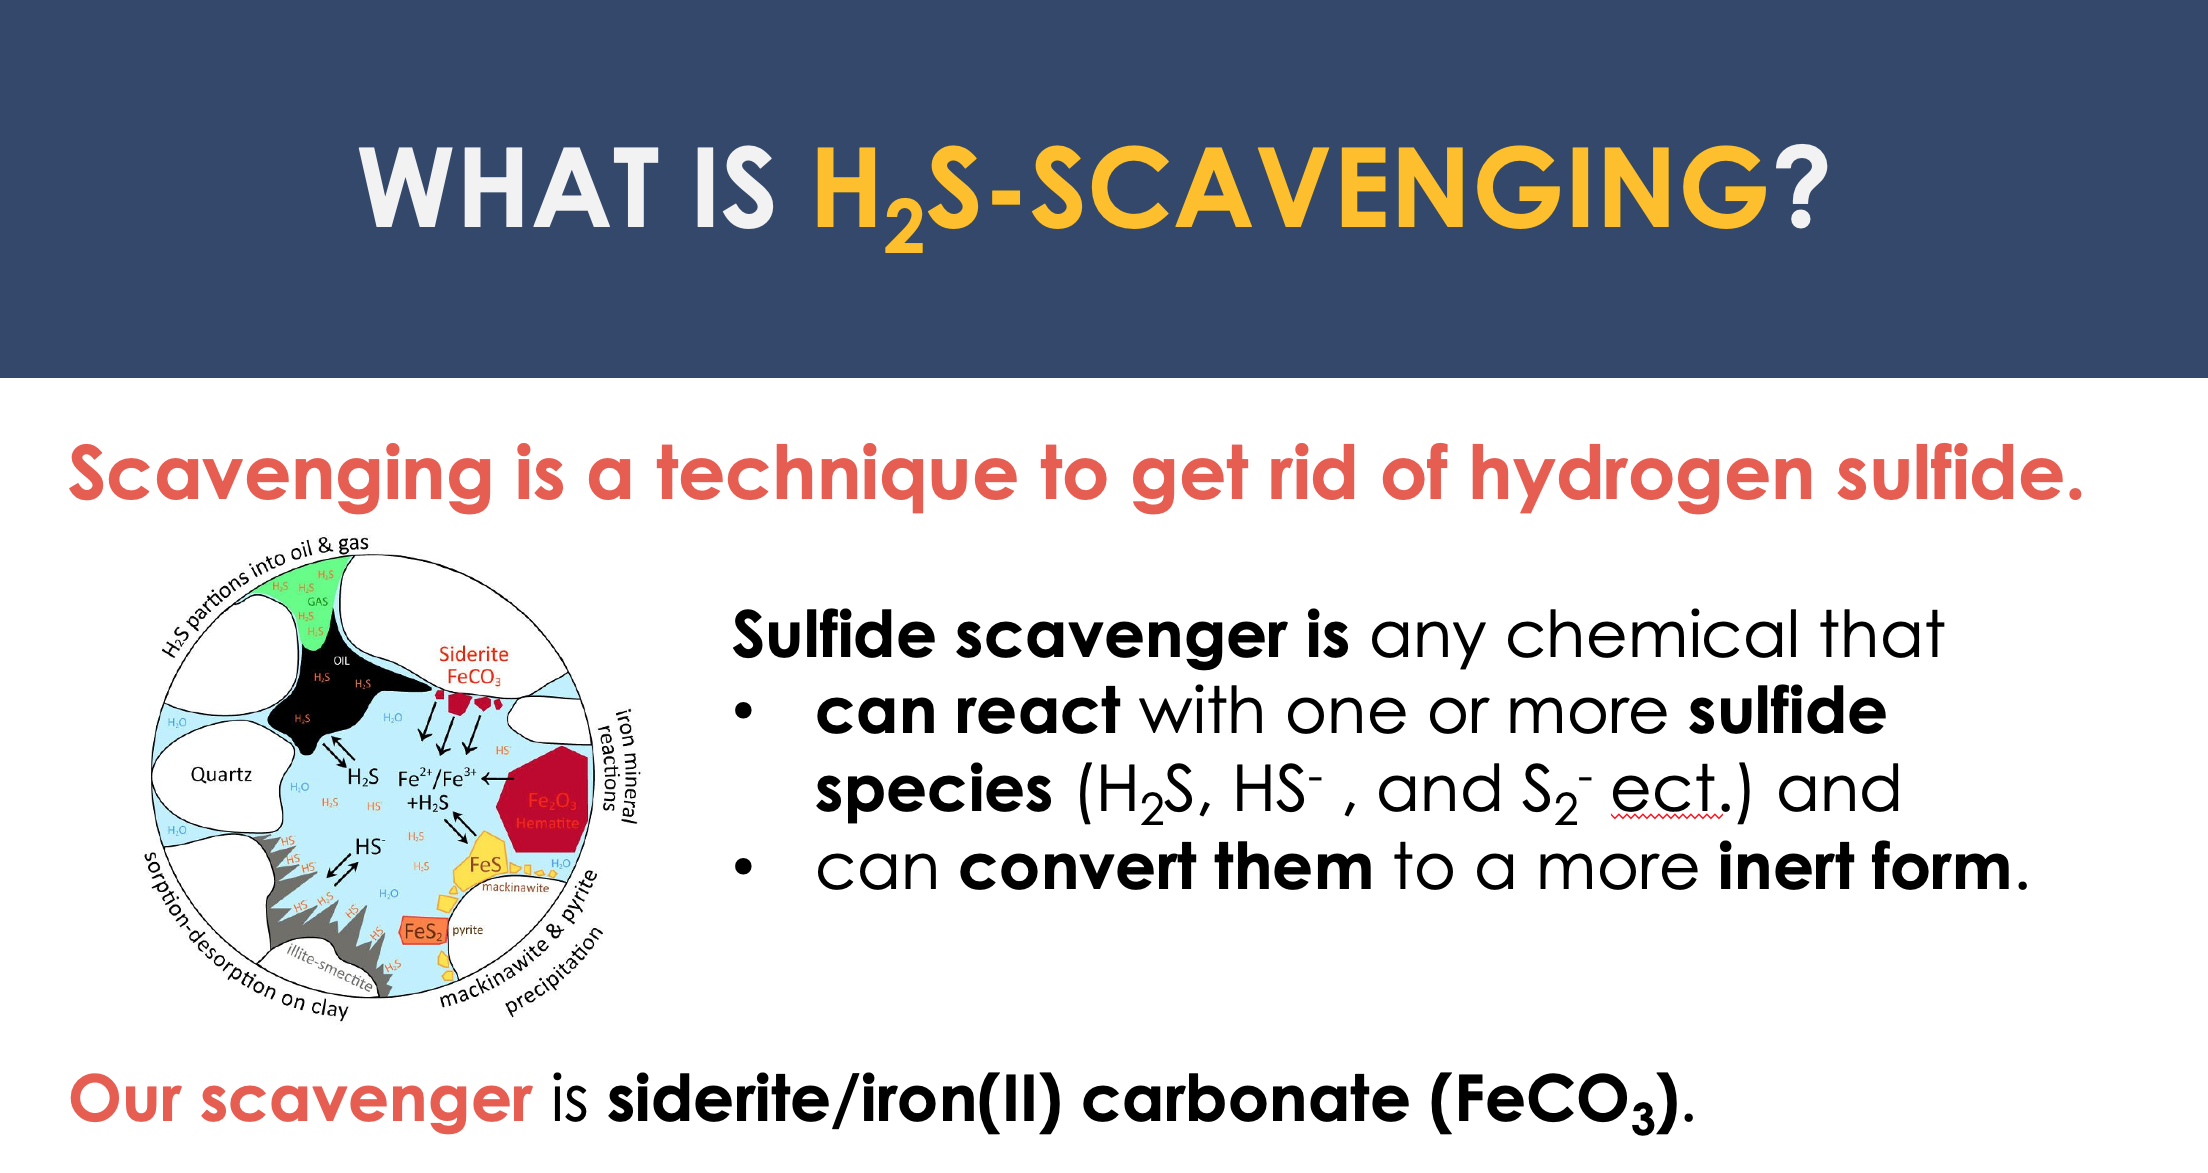
\includegraphics[width=1.0\textwidth]{figures/reactive-transport/scavenging.png}
	%
	\end{figure}
	}
\end{frame}
%
\begin{frame}
	\Wider{
		\vskip 10pt
		\begin{figure}[!t]
			\centering
			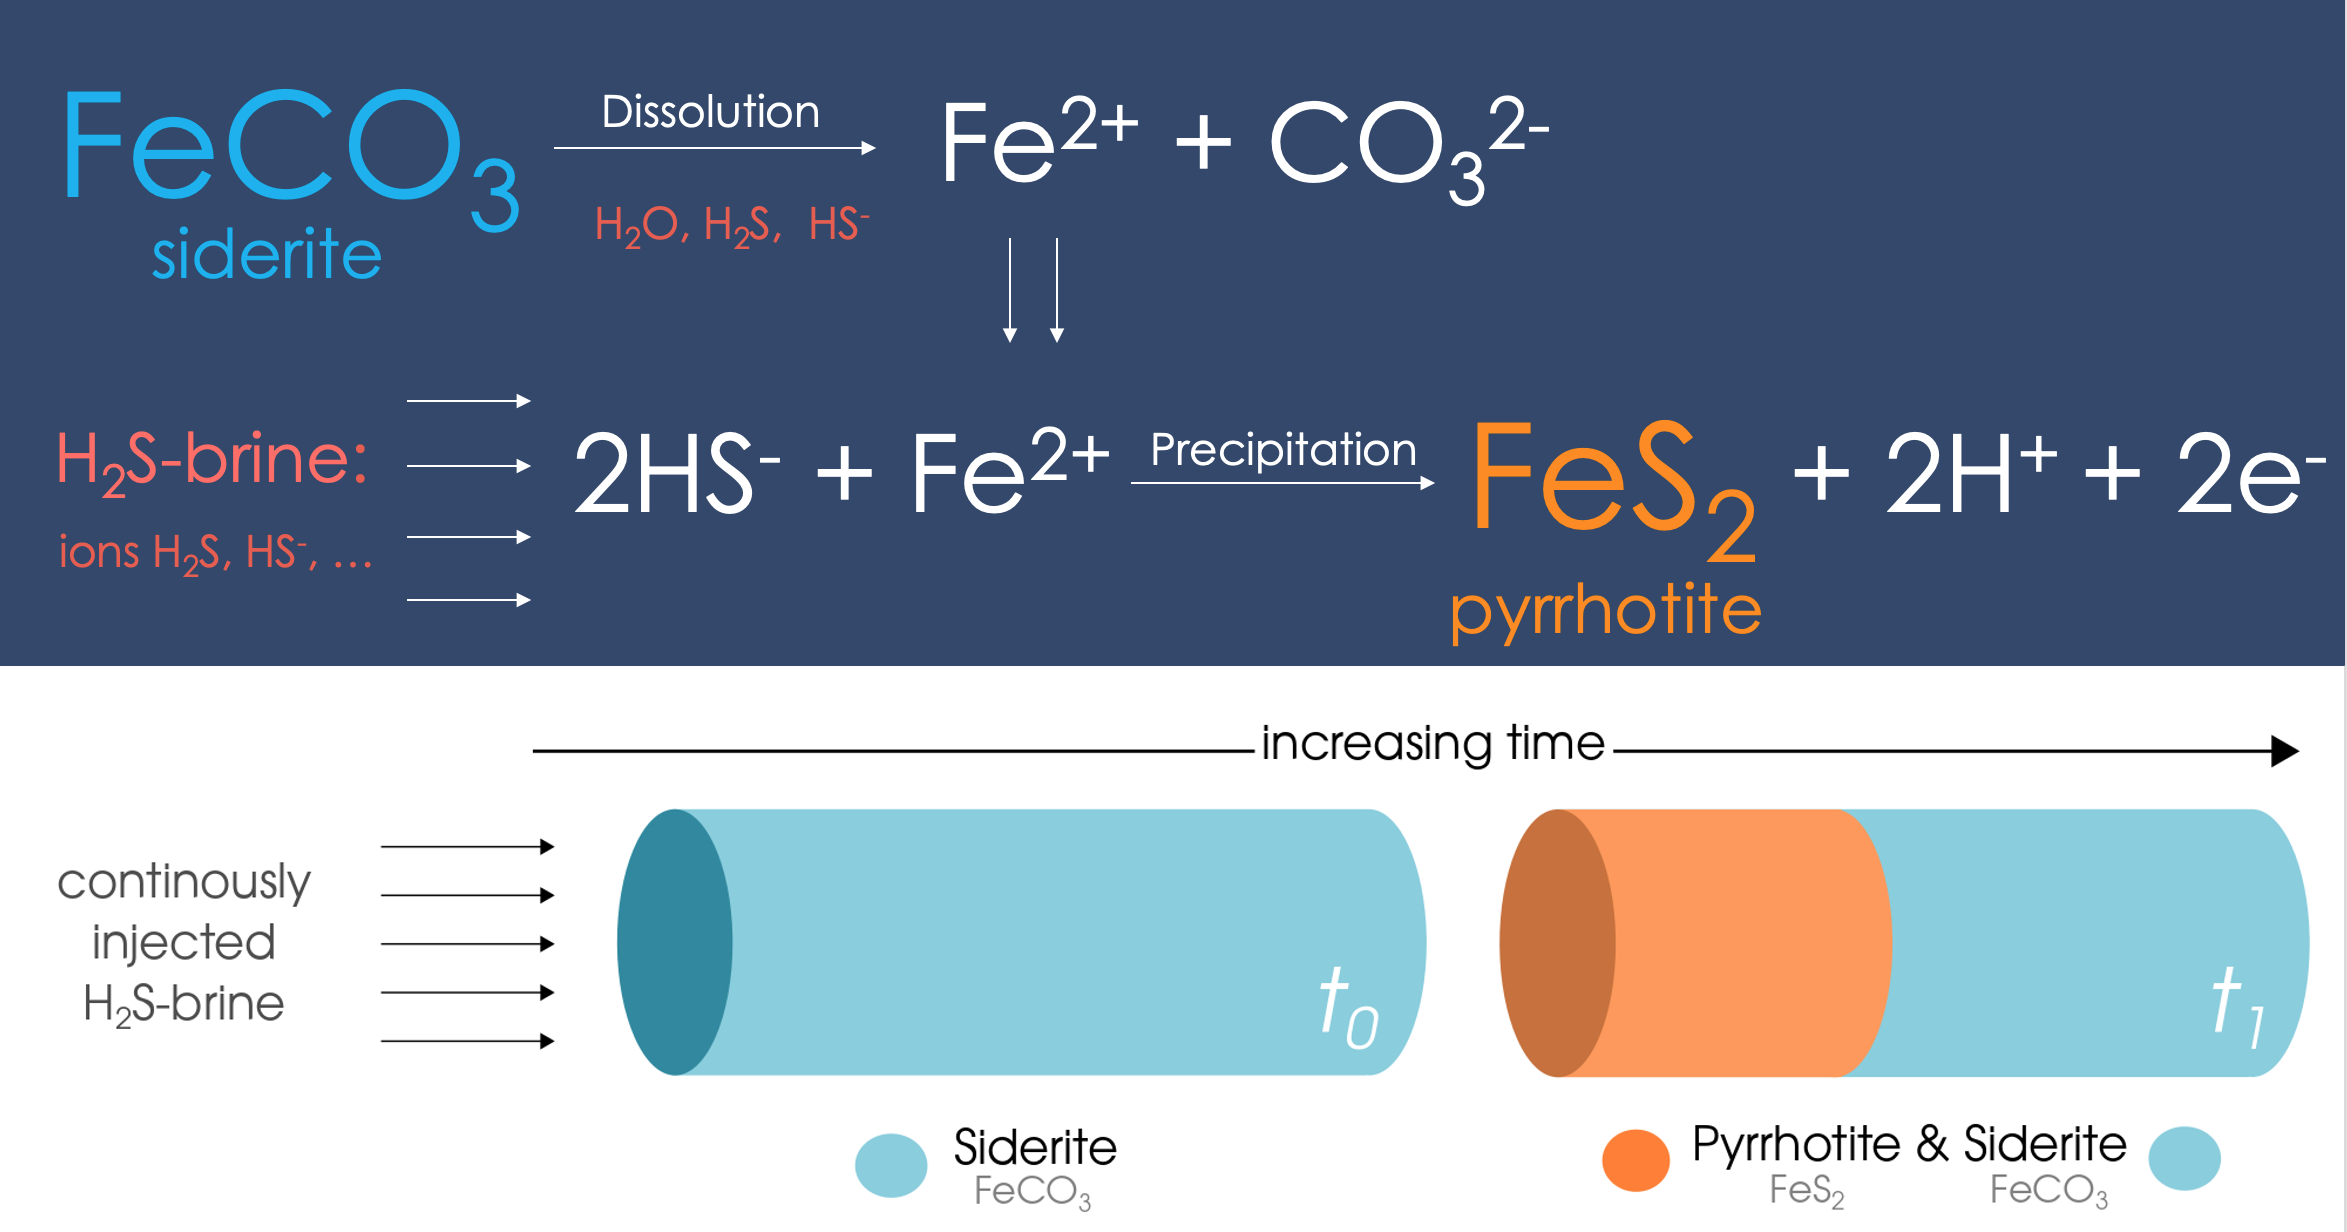
\includegraphics[width=1.0\textwidth]{figures/reactive-transport/souring-reactions.png}
		\end{figure}
	}
\end{frame}
%
\begin{frame}
	\Wider{
		\vskip 10pt
		\begin{figure}[!t]
			\centering
			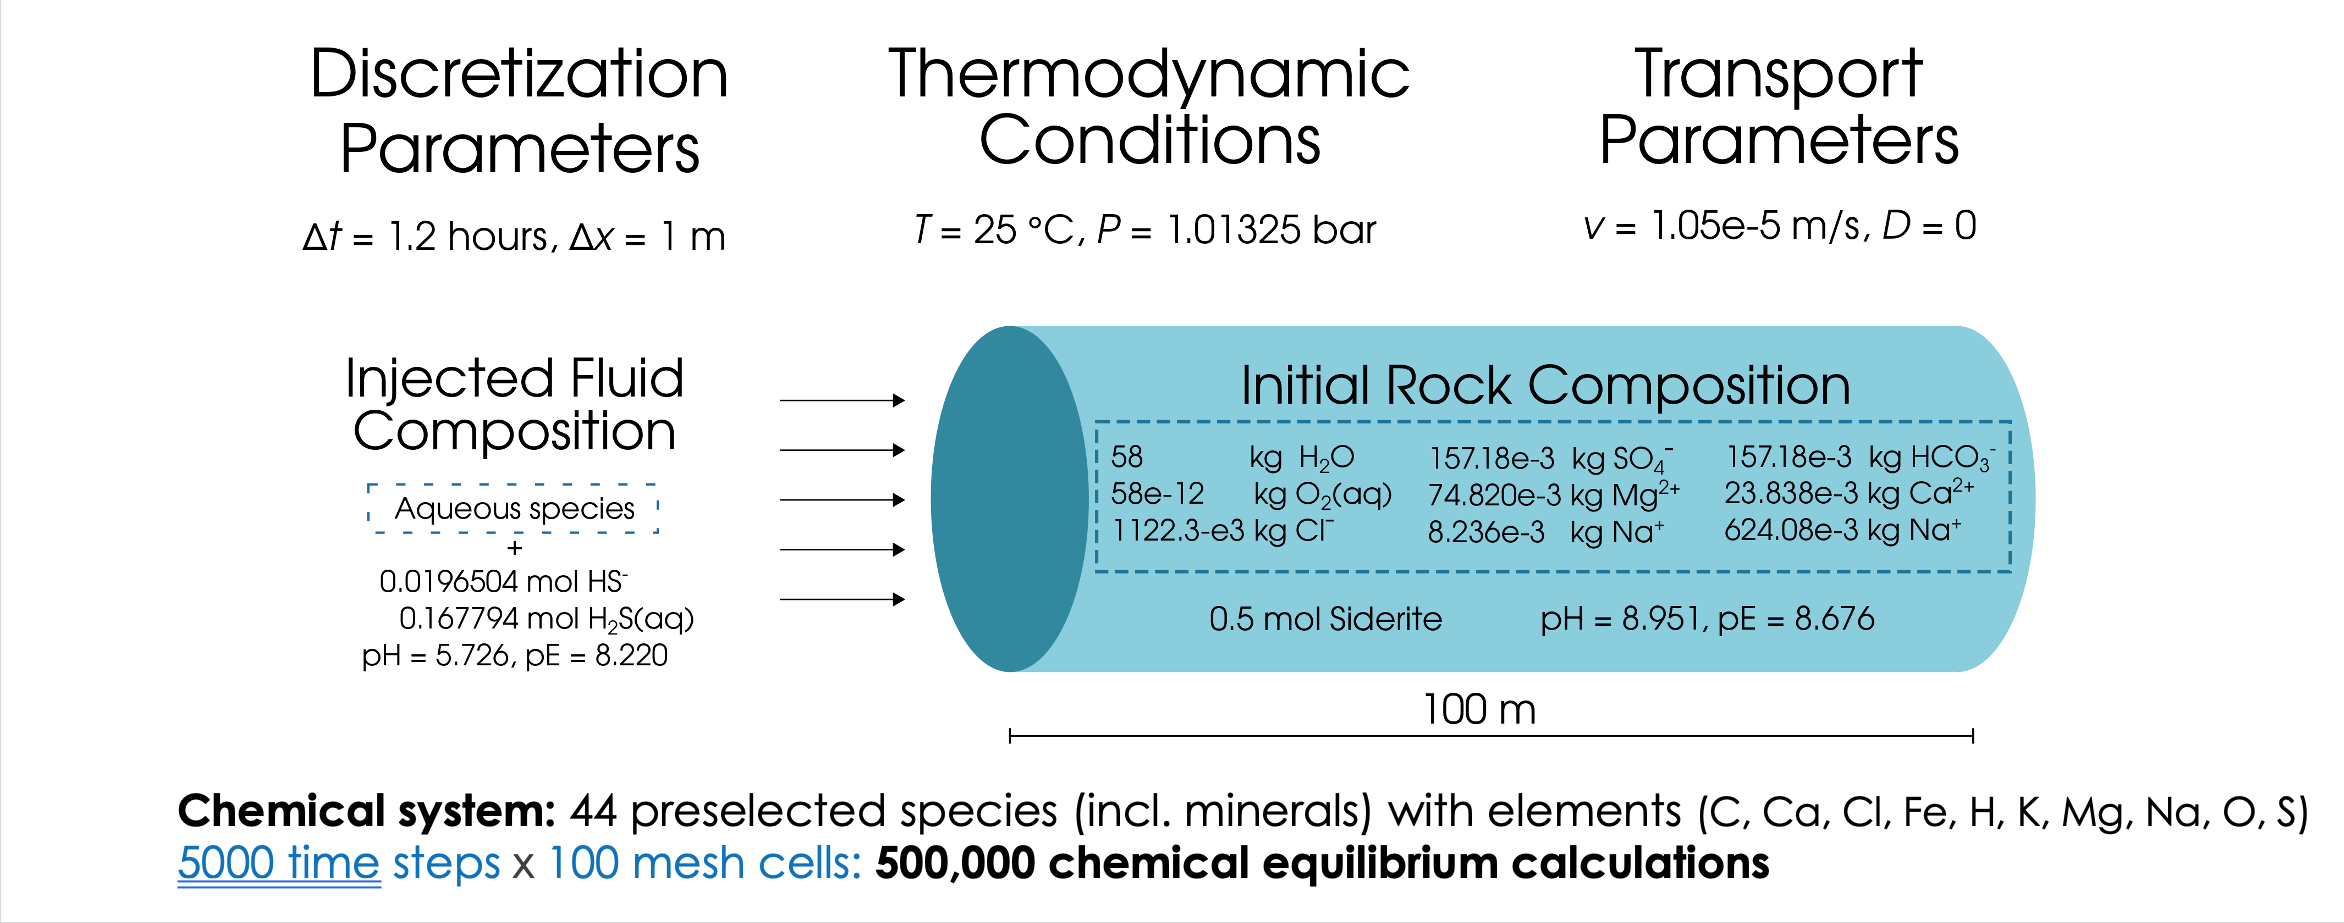
\includegraphics[width=1.0\textwidth]{figures/reactive-transport/souring-discretization.png}
		\end{figure}
	}
\end{frame}
%
\begin{frame}{Example, Results of souring modeling}	
	Jupyter notebook tutorial \href{https://github.com/mtsveta/reaktoro-jupyter/blob/master/tutorial/rt.scavenging.ipynb}{\textcolor{indigo(dye)}{\it RT modeling of the H$_2$S scavenging process along a rock core}}:
	%
	\begin{figure}[!t]%
		\centering
		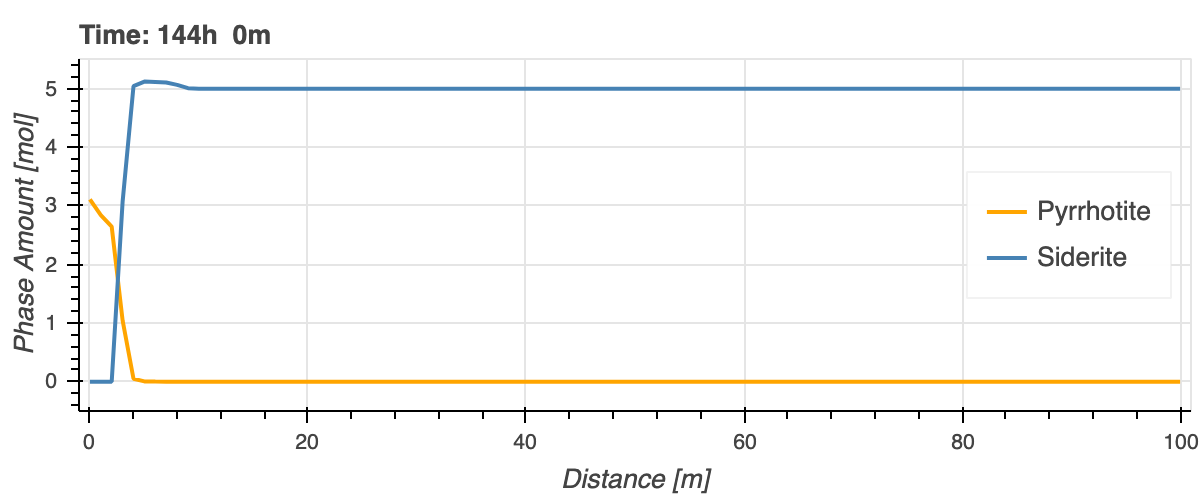
\includegraphics[width=0.54\textwidth]{figures/reactive-transport/siderite-pyrrhotite-1.png} \\
		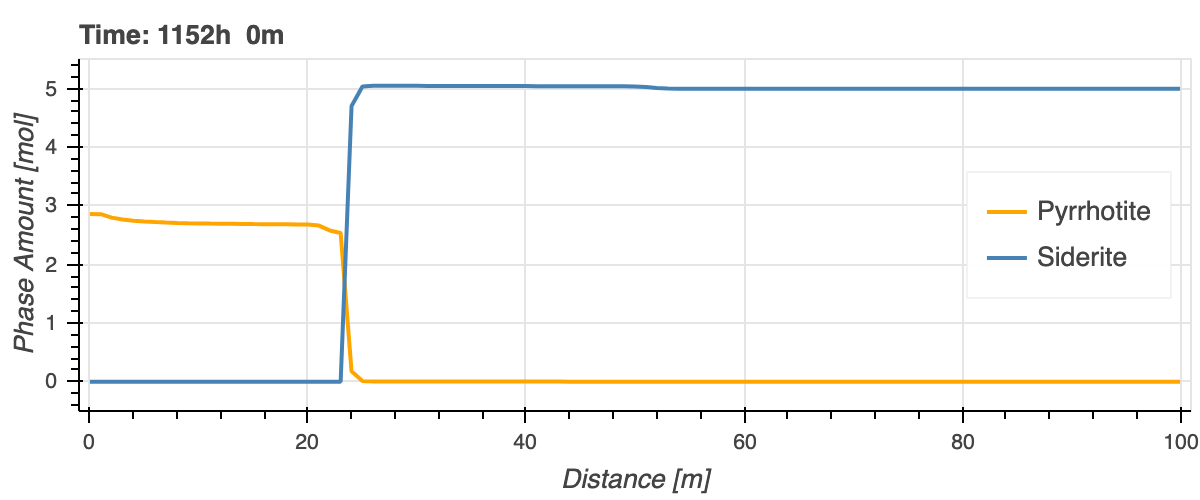
\includegraphics[width=0.54\textwidth]{figures/reactive-transport/siderite-pyrrhotite-2.png}
		\caption{Siderite dissolution and pyrrhotite precipitation.}
	\end{figure}
\end{frame}

%\section{Reactive transport flow}
%
%\begin{frame}{Single-phase fluid flow in porous media}
%%	We consider a relatively simple model for fluid flow for the purpose
%%	of assessing the potential of the ODML algorithm to accelerate chemical
%%	equilibrium calculations in reactive transport simulations. . This
%%	is because our interest in this study is to evaluate how ODML behaves
%%	considering more complex chemical systems and heterogeneous porous
%%	media. In what follows, we assume the fluid is incompressible, gravity
%%	effects are negligible, and the porous medium is isotropic and nondeformable.
%	Solve the coupled \alert{\textbf{continuity equation}}
%	and the  \alert{\textbf{Darcy equation}} below to compute the fluid pressure
%	$P$ and fluid Darcy velocity $\boldsymbol{u}$ throughout the medium:
%	\begin{alignat}{2}
%		\nabla\cdot(\varrho\boldsymbol{u}) & =f & \qquad & \text{in }\Omega\times(0,t_{{\rm final}}),\\
%		\boldsymbol{u} & =-\frac{\kappa}{\mu}\nabla P &  & \text{in }\Omega\times(0,t_{{\rm final}}).\label{eq:darcy}
%	\end{alignat}
%	Here, 
%	\begin{itemize}
%		\item $\varrho$ and $\mu$ are the fluid density and the dynamic
%		viscosity,
%		\item $f$ corresponds to the fluid injection\slash production
%		rate, 
%		\item $\kappa=\kappa(\boldsymbol{x})$, $\boldsymbol{x}\in\Omega$,
%		represents the (isotropic) permeability field of the porous rock,
%		\item $\Omega$ denotes the physical domain, and 
%		\item $t_{{\rm final}}$ indicates the final simulation time.
%	\end{itemize}
%	
%\end{frame}
%
%\begin{frame}{Reactive transport of the fluid species}
%%	Mass conservation applies to the chemical species in the fluid as
%%	they advect, diffuse, disperse, and react with rock minerals in a
%%	porous medium. We apply the mathematical formulation presented in
%%	Appendix~4 of \citet{Allanetal2020} for the reactive transport of
%%	fluid species in terms of mass conservation of chemical elements and
%%	electric charge. This approach is a standard procedure in the literature
%%	that substantially reduces the number of PDEs to be solved for transport
%%	phenomena \citep{Lichtner1985}. 
%%	The formulation also accounts for
%%	the dissolution and precipitation of rock minerals. 
%	For convenience,
%	we write below the governing equation:
%	\begin{equation}
%		\frac{\partial(b_{i}^{\text{f}}+b_{i}^{\text{s}})}{\partial t}+\nabla\cdot(\boldsymbol{v}b_{i}^{\text{f}}-D\nabla b_{i}^{\text{f}})=0\qquad(i=1,\ldots,\mathrm{E}),\label{eq:elemental-mass-conservation-equation}
%	\end{equation}
%	where $b_{i}^{\text{f}}$ and $b_{i}^{\text{s}}$ are the \emph{bulk
%		concentrations }(mol/m$^{3}$)\emph{ of elements(chemical elements
%		and charge) in the fluid and the solid partitions}, respectively\emph{.
%	}Here, $D$ is the \emph{dispersion-diffusion tensor} \citep{Peaceman1977},
%	i.e., 
%	\begin{equation}
%		D=(\alpha_{\mathrm{mol}}+\alpha_{\mathrm{t}}|\boldsymbol{u}|)I+\frac{\alpha_{\mathrm{l}}-\alpha_{\mathrm{t}}}{|\boldsymbol{u}|}\boldsymbol{u}\otimes\boldsymbol{u}\label{eq:dispersion-diffusion-tensor}
%	\end{equation}
%	where $\alpha_{\mathrm{mol}}$ is the molecular diffusion coefficient
%	as well as $\alpha_{\mathrm{l}}$ and $\alpha_{\mathrm{t}}$ are the
%	longitudinal and the transversal dispersion coefficients, respectively.
%	
%	\textbf{Note:} We assume $\alpha_{l}$ and $\alpha_{t}$ be both zero
%	so that $D\equiv\alpha_{\mathrm{mol}}$, which suffices for the numerical
%	investigations of the ODML approach performance in Section~\ref{sec:Results}.
%	
%%	Equation~(\ref{eq:elemental-mass-conservation-equation}) possesses
%%	two advantages when compared to the transport equation formulated
%%	for chemical species:
%%	\begin{itemize}
%%		\item Absence of the reaction term in the convection-diffusion equation,
%%		leaving such concerns to a separate chemical kinetic/equilibrium solver
%%		and easing the coupling procedure.
%%		\item A considerable decrease in the number of unknowns, as the number of
%%		elements E is typically considerably smaller than the number of species
%%		N (see~(\ref{eq:elemental-mass-conservation-equation})).
%%	\end{itemize}
%%	\textbf{Note:} For more than one fluid phase (each with its velocity
%%	field) and different diffusion coefficients for the fluid species,
%%	this simplified transport formulation becomes less straightforward.
%\end{frame}
%
%\begin{frame}{Chemical reactions among fluid species and rock minerals}
%%	In our simulations, homogeneous and heterogeneous chemical reactions
%%	among the species are considered. We adopt a \emph{local chemical
%%		equilibrium model} so that both fluid species and rock minerals 
%%	are in chemical equilibrium at any point in space and time. Because
%%	of transport processes and variations in temperature\slash pressure
%%	(when applicable), the chemical equilibrium states are continually
%%	altered at each point of the domain. For example, a rock mineral may
%%	gradually dissolve as the more acidic fluid passes through that point
%%	in space.
%	
%	In this manner, at every discretized point in space, we solve the
%	Gibbs energy minimization problem:
%	\begin{equation}
%		\min_{n}G(T,P,n)\quad\text{subject to}\quad\left\{ \begin{aligned}An=b\\
%			n\geq0
%		\end{aligned}
%		\right.,\label{eq:gem-problem}
%	\end{equation}
%	to compute the \emph{chemical equilibrium amounts }$n=(n_{1},\ldots,n_{\mathrm{N}})$
%	of the species distributed among all fluid and solid phases in the
%	chemical system. Vector $n$ includes the aqueous species amounts
%	(solute and solvent water) and the mineral amounts composing the porous
%	rock. \textbf{Note: }The given input of this chemical equilibrium
%	problem includes the temperature $T$, pressure $P$, and the amounts
%	of chemical elements $b=(b_{1},\ldots,b_{\mathrm{E}})$ (including
%	electric charge), whereas the constraints include the mass balance
%	$An=b$ and non-negativity of the species amounts $n\geq0$. In~(\ref{eq:gem-problem}),
%	$T$ is assumed to be constant throughout the medium, $P$ computed
%	via the solution of the continuity and Darcy equations, and \textbf{$b$}
%	is updated over time via~(\ref{eq:elemental-mass-conservation-equation}).
%	For more information on solving the GEM problem, we refer to \citet{Leal2017,Allanetal2020}.
%\end{frame}
%
%\begin{frame}{Time staggered operator splitting steps}
%	To solve the time-dependent reactive transport equations in (\ref{eq:elemental-mass-conservation-equation}),
%	we apply the fully discrete formulation typically resulting from a
%	combination of the finite difference approximation in time with the
%	finite element approach in space. We use index$k$ to denote the \emph{time-step}
%	and $\Delta t=t^{k+1}-t^{k}$ to determine the \emph{time-step size.
%	}We assume the uniform discretization $I_{\ensuremath{\Delta t}}:=\{0=t_{0}<t_{1}<...<t_{K}=t_{{\rm final}}\}$
%	of the time interval $[0,t_{{\rm final}}]$, where $t_{{\rm final}}>0$
%	is the total time. \emph{The operator splitting scheme }described
%	below is used to solve these transport equations\emph{:}
%	\begin{enumerate}
%		\item[\textbf{I.}] Consider~(\ref{eq:elemental-mass-conservation-equation}) employing
%		the \emph{backward Euler scheme in time} to compute an auxiliary element
%		concentrations approximation $\tilde{b}_{i}^{\text{f, k+1}}=\tilde{b}_{i}^{\text{f}}(t_{k+1}),$
%		$i=1,\ldots,\text{E}$, in the fluid partition:
%		\begin{equation}
%			\frac{\tilde{b}_{i}^{\text{f},k+1}-\tilde{b}_{i}^{\text{f},k}}{\Delta t}+\nabla\cdot(\boldsymbol{u}\tilde{b}_{i}^{\text{f},k+1}-D\nabla\tilde{b}_{i}^{\text{f},k+1})=0\qquad\text{in}\quad\Omega.x\label{eq:fluid-element-transport}
%		\end{equation}
%		We assume the flux boundary condition on the \emph{inlet face of boundary}
%		$\Gamma_{{\rm inlet}}\subset\partial\Omega$, where we inject the
%		brine,
%		\[
%		-(\boldsymbol{u}\tilde{b}_{i}^{{\rm f},k+1}-D\nabla\tilde{b}_{i}^{{\rm f},k+1})\cdot\boldsymbol{n}_{\text{inlet}}=u\hat{b}_{i,\text{inlet}}\quad\text{on}\quad\Gamma_{\text{inlet}}
%		\]
%		and zero flux on the top and bottom of the boundary, $\Gamma_{\text{top}},\Gamma_{\text{bottom}}\subset\Gamma\equiv\partial\Omega$,
%		\[
%		-(\boldsymbol{u}\tilde{b}_{i}^{{\rm f},k+1}-D\nabla\tilde{b}_{i}^{{\rm f},k+1})\cdot\textbf{\emph{\ensuremath{\boldsymbol{n}}}}=0\quad\text{on}\quad\Gamma_{\text{top}}\cup\Gamma_{\text{bottom}}.
%		\]
%		The right boundary is considered a free outflow boundary. Vector $\boldsymbol{n}$
%		denotes the outward-pointing normal to the boundary face $\Gamma$
%		($\boldsymbol{n}_{\text{inlet}}$ is the normal on $\Gamma_{\text{inlet}}$),
%		and $\hat{b}_{i,\text{inlet}}$ (in $\mathrm{mol/m_{\mathrm{fluid}}^{3}}$)
%		represents the given concentration of the injected brine. As a space
%		discretization solver for~(\ref{eq:fluid-element-transport}), we
%		employ the Streamline-Upwind Petrov-Galerkin (SUPG) scheme introduced
%		in \citet{BrooksHughes} (see Section~\ref{subsec:supg-method})
%		to handle advection-dominated transport in a accurate and stable way.
%		
%		The velocity in~(\ref{eq:fluid-element-transport}) is generated
%		from the coupling to the Darcy problem, i.e., $\boldsymbol{u}=\boldsymbol{u}^{k}$,
%		where $\boldsymbol{u}^{k}$ satisfies the system
%		\begin{equation}
%			\begin{array}{cccc}
%				\nabla\cdot(\varrho\boldsymbol{u}^{k}) & = & f^{k} & {\rm in}\quad\Omega\times(0,t_{{\rm final}}),\\
%				\boldsymbol{u}^{k} & = & -\tfrac{\kappa}{\mu}\nabla P^{k} & {\rm in\quad\Omega\times(0,t_{{\rm final}}).}
%			\end{array}\label{eq:darcy-discretized}
%		\end{equation}
%		A comprehensive numerical analysis, demonstrating the existence and
%		uniqueness of the solution for the prior semi-discrete system, can
%		be found in \citet{MaltaLoula1998,Maltaetal2000}.
%		\item[\textbf{II.}] Evaluate the total element concentrations $b_{i}$, using prior reconstructed
%		$\tilde{b}_{i}^{\text{f},k+1}$ and $b_{i}^{\mathrm{s}}$ (assumed
%		constant) : 
%		\[
%		b_{i}^{k+1}=\tilde{b}_{i}^{\text{f},k+1}+b_{i}^{\text{s},k}.
%		\]
%		\item[\textbf{III.}] In each space discretization cell, calculate $n^{k+1}$ for given
%		\emph{T, P,} and\emph{ }$b^{k+1}$ using the smart chemical equilibrium
%		algorithm accelerated with the ODML strategy (see Section~\ref{subsec:First-order-Taylor-approximation}).
%	\end{enumerate}
%	To make sure that the Courant–Friedrichs–Lewy (CFL) condition is satisfied,
%	we assume ${\mathrm{CFL}=0.3}$ and the time step is defined by
%	\begin{equation}
%		\Delta t=\frac{{\rm CFL}}{\max\Big\{\max|v_{x}|/\Delta x,\,\max|v_{y}|/\Delta y\Big\}},
%	\end{equation}
%	where $v=[v_{x};v_{y}]^{{\rm T}}$, and $\Delta x$ and $\Delta y$
%	are the lengths of the cells along the $x$ and $y$ coordinates,
%	respectively.
%	
%\end{frame}